\documentclass{newsiambook}
\usepackage{makeidx}
\usepackage{epic}
\usepackage{curves}
\usepackage{amsmath}
\usepackage{amssymb}
\usepackage{longtable}
%\usepackage{color}
 \usepackage{thumbpdf}
 \usepackage[pdftex]{color} % black,white,red,green,blue,cyan,magenta,yellow
 \usepackage[pdftex,colorlinks]{hyperref}
 \usepackage[pdftex]{graphicx}
 \usepackage{float}


%%% this centers the text on a letter size page
\setlength{\oddsidemargin}{0.0in}
\setlength{\evensidemargin}{0.016in}

%%% this makes the left margin bigger
%%% (pages match for two sided printing)
%\setlength{\oddsidemargin}{0.75in}
%\setlength{\evensidemargin}{-0.734in}

%%% these are the default settings in newsiambook.cls
%%% (pages match for one sided printing)
%\setlength{\oddsidemargin}{.75in}
%\setlength{\evensidemargin}{.766in}

\def\mb#1{\mbox{\boldmath $#1$}}
\def\norm#1{|\!| #1 |\!|}
\def\bignorm#1{\big|\!\big| #1 \big|\!\big|}
\def\biggnorm#1{\bigg|\!\bigg| #1 \bigg|\!\bigg|}
\def\Bignorm#1{\Big|\!\Big| #1 \Big|\!\Big|}
\def\Biggnorm#1{\Bigg|\!\Bigg| #1 \Bigg|\!\Bigg|}
\def\snorm#1{| #1 |}
\def\bigsnorm#1{\big| #1 \big|}
\def\biggsnorm#1{\bigg| #1 \bigg|}
\def\Bigsnorm#1{\Big| #1 \Big|}
\def\Biggsnorm#1{\Bigg| #1 \Bigg|}
\def\enorm#1{|\!|\!| #1 |\!|\!|}
\def\bigenorm#1{\big|\!\big|\!\big| #1 \big|\!\big|\!\big|}
\def\biggenorm#1{\bigg|\!\bigg|\!\bigg| #1 \bigg|\!\bigg|\!\bigg|}
\def\Bigenorm#1{\Big|\!\Big|\!\Big| #1 \Big|\!\Big|\!\Big|}
\def\Biggenorm#1{\Bigg|\!\Bigg|\!\Bigg| #1 \Bigg|\!\Bigg|\!\Bigg|}
\def\Re{I\!\!R}
\def\eref#1{(\ref{#1})}

\def\tab{\par\indent}
\def\tabb{\tab\hskip1.5em}
\def\tabbb{\tab\hskip3.5em}
\def\atab#1{\par\indent\hskip5.0em{\bf  #1}\hskip1.5em}
\def\ctab{\par\indent\hskip8.5em}
\newenvironment{plt}{\vspace{0.1cm}\footnotesize}{\normalsize \vspace{0.1cm}}
\newenvironment{plt0}{\vspace{0.1cm}}{\vspace{0.1cm}}
\newenvironment{qqt}{\vspace{0.1cm}\begin{quote}}{\end{quote} \vspace{0.1cm}}
\newenvironment{lst}{\begin{itemize} \itemsep=0pt}{\end{itemize}}
\def\f#1{\textsl{#1}}
\def\ff#1{\mbox{\textsl{#1}}}

% peg's spacing in tables

\newcommand{\strutul}{\rule[-1ex]{0pt}{3.5ex}}%   Total height 3.5
\newcommand{\strutl}{\rule[-1ex]{0pt}{2.5ex}}%    Total height 3.5
\newcommand{\strutu}{\rule[-.5ex]{0pt}{3ex}}%     Total height 3.5

% colors etc

%\definecolor{myblue}{rgb}{0.375,0.375,0.75}
\definecolor{myblue}{rgb}{0.2,0.2,0.7}
\definecolor{mygreen}{rgb}{0,0.6,0}
\definecolor{mycyan}{rgb}{0,0.6,0.6}
\definecolor{myred}{rgb}{0.9,0.2,0.2}
\definecolor{mymagenta}{rgb}{0.9,0.2,0.9}

\def\Blue#1{{\color{myblue}#1}}
\def\Red#1{{\color{myred}#1}}
\def\Green#1{{\color{mygreen}#1}}
\def\Cyan#1{{\color{mycyan}#1}}
\def\Magenta#1{{\color{mymagenta}#1}}



%%%%%%%%%%%%%%%%%%%%%%%%%%%%%%%%%%%%%%%%%%%%%%%%%%%%%%%%%%%%%%%%%%%%%%%%%%%%%%
\newif\ifpdf
\ifx\pdfoutput\undefined
   \pdffalse        % running LaTeX
\else
 \ifcase\pdfoutput
    \pdffalse       % running LaTeX
 \else
    \pdftrue        % running pdfLaTeX
 \fi
\fi

\def\myfig#1#2{\includegraphics[height=#1] {#2}}
%%%%%%%%%%%%%%%%%%%%%%%%%%%%%%%%%%%%%%%%%%%%%%%%%%%%%%%%%%%%%%%%%%%%%%%%%%%%%%



%\psdraft
\makeindex
\begin{document}
\pagenumbering{roman}
\setcounter{page}{1}
\markboth{WEBGUI USERS' GUIDE}{CONTENTS}

\begin{titlepage}
\begin{flushleft}
{\sffamily{\Huge{\bfseries{
        WEBGUI:}}}}\\
{\sffamily{\huge{\bfseries{
	A Web Browser Based\\
        Graphical User Interface\\
        for Scientific Software\\ }}}}
\vspace*{0.4cm}
{\sffamily{\huge{\bfseries{
        Users' Guide}}}}\\
\vspace{0.6cm}
{\sffamily\LARGE{
Christopher Deotte\\}}
\vspace{0.2cm}
{\sffamily\Large{
Department of Mathematics \\
University of California at San Diego \\
La Jolla, California 92093-0112\\
\vspace{0.6cm}
June, 2017}\\
}
\end{flushleft}
\end{titlepage}
\newpage

%\thispagestyle{empty}
\begin{flushleft}
\vspace*{3.0cm}
{\sffamily\large{
Copyright (c) 2017, Christopher Deotte.}}\\
\vspace{0.5cm}
{\sffamily\large{
This work was supported by the National Science Foundation \\
under grant DMS-1345013.}} \\
\vspace{1.0cm}
{\sffamily\normalsize{
  Permission is hereby granted, free of charge, to any person obtaining a copy
of this software and associated documentation files (the "Software"), to deal
in the Software without restriction, including without limitation the rights
to use, copy, modify, merge, publish, distribute, sublicense, and/or sell
copies of the Software, and to permit persons to whom the Software is
furnished to do so, subject to the following conditions:\\
\vspace{0.5cm}
The above copyright notice and this permission notice shall be included in all
copies or substantial portions of the Software.\\
\vspace{0.5cm}
THE SOFTWARE IS PROVIDED "AS IS", WITHOUT WARRANTY OF ANY KIND, EXPRESS OR
IMPLIED, INCLUDING BUT NOT LIMITED TO THE WARRANTIES OF MERCHANTABILITY,
FITNESS FOR A PARTICULAR PURPOSE AND NONINFRINGEMENT. IN NO EVENT SHALL THE
AUTHORS OR COPYRIGHT HOLDERS BE LIABLE FOR ANY CLAIM, DAMAGES OR OTHER
LIABILITY, WHETHER IN AN ACTION OF CONTRACT, TORT OR OTHERWISE, ARISING FROM,
OUT OF OR IN CONNECTION WITH THE SOFTWARE OR THE USE OR OTHER DEALINGS IN THE
SOFTWARE.}}\\
\end{flushleft}

\newpage

 \tableofcontents

 \cleardoublepage
\setcounter{chapter}{-1} %The counter for chapters should be set one less than 
                        %the actual chapter number, for example, {1} for 
                        %chapter 2, and {2} for chapter 3.
\setcounter{section}{0} %The counter for sections should be set to match the
                        %actual chapter number, for example, {2} for sections 
                        %in chapter, and {3} for sections in chapter 3. 
%\chapter*{Preface}
\chapter*{\begin{flushleft}  Preface \end{flushleft}}
\addcontentsline{toc}{chapter}{Preface}
\label{preface}
\markboth{WEBGUI USERS' GUIDE}{PREFACE}
\pagenumbering{roman}
\setcounter{page}{5} %The counter for page numbers must be placed here in your
                     %chapter, following the \chapter and \markboth commands.
                     %It should always be the next available right-hand page.
                     %All chapters start on new rights. It will always be
                     %an odd number.  


The idea for \f{WEBGUI} came from Randolph E. Bank and Michael Holst of the University
of California at San Diego. They each have existing scientific software (PLTMG and FETK
respectively) and they wanted a graphical user interface (GUI) that was platform independent and
could control their software either locally or remotely. They suggested building a GUI that
displayed in a web browser. It has been my great pleasure to create this \f{WEBGUI}. 
 
This version of \f{WEBGUI} was supported by the National Science Foundation
through grant DMS-1345013.

\vspace{5mm}
\noindent {\em University of California at San Diego}\hfill Christopher Deotte\\
{\em June, 2017}











 \newpage
 \cleardoublepage
\setcounter{chapter}{0} %The counter for chapters should be set one less than 
                        %the actual chapter number, for example, {1} for 
                        %chapter 2, and {2} for chapter 3.
\setcounter{section}{1} %The counter for sections should be set to match the
                        %actual chapter number, for example, {2} for sections 
                        %in chapter, and {3} for sections in chapter 3. 

\chapter{Introduction}
\label{intro}
\markboth{WEBGUI USERS' GUIDE}{INTRODUCTION} %For running heads. The first 
         %field will be the same for every chapter. The second will contain the 
         %appropriate chapter title.
\pagenumbering{arabic}
\setcounter{page}{1} 

\section{Description}

\f{WEBGUI} is a C language library that creates for your software a graphical user interface (GUI) after
only a few library function calls. \f{WEBGUI} is platform independent because it displays everything
in any standard web browser. And \f{WEBGUI} allows the interface to reside on either the local machine
or a remote machine.
 

\section{Overview}

\f{WEBGUI} works by enabling your program to mimic a web server. When your program calls the library
routine "webstart(int x)", a new thread is created which sets up a web server and begins listening on port x.  
Both your program and the web server run on the same host machine. Using any standard web browser either 
locally or remotely, enter the URL of the host machine. Then, the web browser will display a set of controls. 
The web browser is in constant communication with
your software running on the host machine. All of your software's output will be displayed in the web
browser and all input you provide in the web browser will be sent to your software.

\section{Installation}

Simply compile and link \f{WEBGUI} to your program. No other files are needed. For example, 
"gcc YourProgram.c webgui.c". To start the service, call the routine "webstart(int port)" within your program. 
Next, to send text output to the web browser, call the routine "writeline(char* str)" where str is a string of length 80. 
To receive input, call the routine "readline(char* str)" where str is a buffer that can receive a string of length 80.
Lastly, to display 2D images, or 3D objects, call either "webimagedisplay" or "webgldisplay".
If you would like your web browser controls to have buttons, call the routine "webinit". To learn more
about these and other routines, read Chapter \ref{chap:2} titled, "WebGUI API" below.

 \newpage
 \cleardoublepage
\setcounter{chapter}{1} %The counter for chapters should be set one less than 
                        %the actual chapter number, for example, {1} for 
                        %chapter 2, and {2} for chapter 3.
\setcounter{section}{2} %The counter for sections should be set to match the
                        %actual chapter number, for example, {2} for sections 
                        %in chapter, and {3} for sections in chapter 3. 
\chapter{WebGUI API}
\label{chap:2}
\markboth{WEBGUI USERS' GUIDE}{WEBGUI API}
\pagenumbering{arabic}
\setcounter{page}{3} %The counter for page numbers must be placed here in your
                     %chapter, following the \chapter and \markboth commands.
                     %It should always be the next available right-hand page.
                     %All chapters start on new rights. It will always be
                     %an odd number.  

 
\section{Overview}

\f{WEBGUI} has 19 available functions organized into 4 categories. Each is described in its own section below.\\
\\
\underline{Basic control:}\\
int webstart(int port)\\
void webwriteline(char* str)\\
void webreadline(char* str)\\
void webinit(char* str, int len)\\
void webupdate(int* ip, double* rp, char* sp)\\
void websettitle(char* str)\\
void webstop()\\
\\
\underline{2D Image display:}\\
void websetcolors(int nc, double* R, double* G, double* B, int pane)\\
void webimagedisplay(int nx, int ny, int* image, int pane)\\
\\
\underline{3D Object display:}\\
void websetcolors(int nc, double* R, double* G, double* B, int pane)\\
void webframe(int frame)\\
void weblineflt(float* x, float* y, float* z, int n, int color)\\
void webfillflt(float* x, float* y, float* z, int n, int color)\\
void weblinedbl(double* x, double* y, double* z, int n, int color)\\
void webfilldbl(double* x, double* y, double* z, int n, int color)\\
void webgldisplay(int pane)\\
\\
\underline{Miscellaneous:}\\
int webquery()\\
void webbutton(int highlight, char* cmd)\\
void webpause()\\
void websetmode(int x)\\

\section{Compiling and linking}
The only file that you need to compile and link to your software is webgui.c. No other files are needed. It is true that webgui.c 
mimics a web server and transmits index.html and 3 png images, but these 4 resources are contained within the webgui.c
file as C data.

You can link and subsequently call the external functions of \f{WEBGUI} from any programming language that can
call C language functions. This library has been tested to work with C and Fortran. Compiling, linking, and calling from C
is straight forward. If you wish to compile, link, and call from Fortran, here are some notes.

Every routine described in this section has a matching routine that accepts all the arguments passed as pointers.
For example, the routine \textbf{webstart(int port)} requires that the integer \textbf{port} is passed by value. However
there exists a routine  \textbf{webstart\_(int* port)}  that accepts \textbf{port} as a pointer. All of the twin routines
that accept pointer references have the same function name as the original but end with an underscore.

These matching twin functions are particularly helpful for linking against Fortran. By default, Fortran calls subroutines
by passing pointers for everything. Even if you call \textbf{webstart(15000)} in Fortran, then Fortran will place
the integer 15000 somewhere in memory and pass a pointer to where it resides. That being said, if you wish to link
\f{WEBGUI} to Fortran, you do not need to write an underscore after each routine name. The compiler does this without
you knowing. Here is an example of how you would call \textbf{webstart} with Fortran:
\begin{verbatim}
integer(kind=4) :: port
port = 15000
call webstart(port)
\end{verbatim}
Notice that the call to \textbf{webstart} does not contain a trailing underscore. However the compiler and linker will look
and link this Fortran call to the \f{WEBGUI} routine \textbf{webstart\_} for you.

Fortran differs from C in other ways also. Fortran accesses arrays
starting from index 1 instead of 0. Whenever this is relevent to a routine it is noted in the API. Namely, the routine \textbf{websetcolors}
defines a palette that you later reference from \textbf{webimagedisplay}, \textbf{webline}, and \textbf{webfill}. When referencing
the colors, you refer to the first color as 0 and the second as 1, etc. This is mentioned in the API below. Also, when calling \textbf{webinit}
you declare indices for the parameters. These indices need to match array indices of arguments to \textbf{webupdate}. In this case,
you start indexing from 1. This is explained in the API to follow.

Fortran does not terminate strings (character arrays) with a NULL (char = 0) like C does. Instead Fortran adds space characters
to fill the entire character array after the used portion of the array. All of \f{WEBGUI}'s routines that accept strings will
accept either C or Fortran strings. These routines are \textbf{webwriteline}, \textbf{webinit}, \textbf{webupdate}, \textbf{websettitle},
and \textbf{webbutton}.

If you wish to compile and link against a Fortran program, type something like
\begin{verbatim}
gcc -c webgui.c
gfortran YourProgram.f webgui.o 
\end{verbatim}

When passing arguments, note that the C language variables \textbf{int, float, double, char[80]} are usually 4, 4, 8, 80 bytes 
respectively. When declaring Fortran variables to use as arguments to call \f{WEBGUI} functions, they must be of compatible size. 
To match the former C variables, one typically declares
 \textbf{integer(kind=4), real(kind=4), real(kind=8), character(len=80)} in Fortran respectively. If you wish to capture a return value
 from one of \f{WEBGUI}'s functions, you must make a Fortran function call instead of a Fortran subroutine call and you must declare
 the return value type.
 
 For example, earlier in this section there is an example showing how to call \textbf{webstart} as a Fortran subroutine. To capture
 the return value from \textbf{webstart}, call it as a Fortran function like the following:
 \begin{verbatim}
integer(kind=4) :: webstart
integer(kind=4) :: error 
integer(kind=4) :: port
port = 15000
error = webstart(port)
\end{verbatim}

\newpage
\section{Basic control}
%%%%%%%%%%%%%%%%%%%%%%%%%%%%%%%%%%%%%%%%%%%%%%%%%%%%%%%%%%%%%%%%%%%%%%%%%%%%
% WEBSTART
%%%%%%%%%%%%%%%%%%%%%%%%%%%%%%%%%%%%%%%%%%%%%%%%%%%%%%%%%%%%%%%%%%%%%%%%%%%%
\subsection{webstart}
\underline{Description} The function \textbf{int webstart(int port)} commences the graphical user interface. Specifically
it deploys a web server and creates a new thread which listens for incoming connections on the chosen port.
After calling \textbf{webstart}, any web browser can connect and display the GUI controls by entering your host
computer's URL:port. Afterward, inside the web browser, they will see a pane for displaying text output, three 
panes for displaying graphical output, and either buttons or a space where they can enter string commands. See Figure
\ref{fig:1}. If you wish to have buttons in your GUI, you need to call \textbf{webinit} before this. See Section \ref{sec:2-1}\\
\\
\underline{Declaration} 
\begin{verbatim} 
	int webstart(int port) 
\end{verbatim}
\underline{Parameters} \textbf{port} is a (4 byte) integer which defines which port the web server will listen on.\\
\\
\underline{Return Value} If successful, 0 is returned. On failure, a negative number is returned. -1 indicates that the
requested port is already in use. -2 indicates an inability to create a socket.\\
\\
\underline{Example} The following example shows the usage of \textbf{webstart}.
\begin{verbatim}
#include <webgui.h>
#include <unistd.h>

int main(){
    webstart(15000);
    pause();
    return 0;
}
\end{verbatim}
Assume that your computer's ip address is 172.217.5.206, then after compiling and running the above program.
You can open any web browser and enter the URL = http://172.217.5.206:15000 and your web browser will
display basic controls as displayed in Figure \ref{fig:1}. If your web browser and program are both running
on the same computer, you can use the URL = http://localhost:15000. After calling \textbf{webstart}, the host machine's 
standard output will display:
\begin{verbatim}
webgui: Listening on port 15000 for web browser...
\end{verbatim}
Or you may see the message:
\begin{verbatim}
webgui: FAILURE: server can't bind port 15000
\end{verbatim}
A common \textbf{webstart} error is trying to run two instances of \textbf{WEBGUI} using the same port. 
The second instance will fail. In this case, \textbf{webstart} returns -1. Your 
software should check for this error and act accordingly. Three suggestions are (i) terminate your program,
(ii) wait 5 seconds and try again, or (iii) try binding to a different port. Here is C code that replaces the line 
\textbf{webstart(15000)} in the above example:\\
case i:
\begin{verbatim}
    if (webstart(15000)<0) exit(1);
\end{verbatim}
case ii:
\begin{verbatim}
    while (webstart(15000)<0) sleep(5);
\end{verbatim}
case iii:
\begin{verbatim}
    int offset=0;
    while (webstart(15000+offset)<0) offset++;
\end{verbatim}
In Fortran, you must declare \textbf{webstart} as a 4 byte integer. Here is Fortran code:\\
case i:
\begin{verbatim}
    integer(kind=4) :: webstart
    if (webstart(15000)<0) stop;
\end{verbatim}
case ii:
\begin{verbatim}
    integer(kind=4) :: webstart
    do
        if (webstart(15000)==0) exit;
        call sleep(5)
    end do
\end{verbatim}
case iii:
\begin{verbatim}
    integer(kind=4) :: webstart, offset
    offset=0
    do
        if (webstart(15000+offset)==0) exit;
        offset = offset+1
    end do
\end{verbatim}

\begin{figure}[p!]
\centering
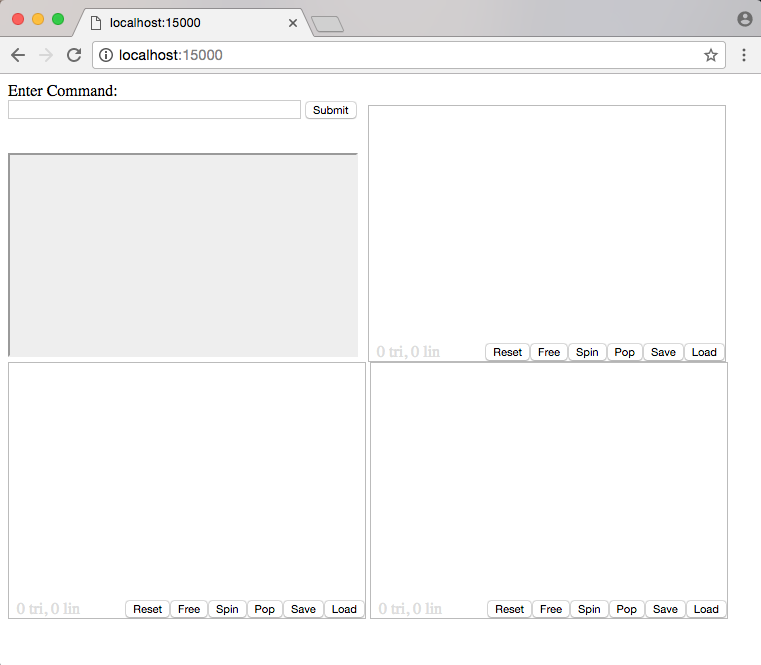
\includegraphics[width=0.75\textwidth]{pix/gui.png}
\caption{\f{WEBGUI} after calling \textbf{webstart}.}
\label{fig:1}
\end{figure} 

%%%%%%%%%%%%%%%%%%%%%%%%%%%%%%%%%%%%%%%%%%%%%%%%%%%%%%%%%%%%%%%%%%%%%%%%%%%%
% WEBWRITELINE
%%%%%%%%%%%%%%%%%%%%%%%%%%%%%%%%%%%%%%%%%%%%%%%%%%%%%%%%%%%%%%%%%%%%%%%%%%%%
\newpage
\subsection{webwriteline}
\label{sec:2-2}
\underline{Description} The function \textbf{void webwriteline(char* str)} displays a line of text in the text
output pane of the web browser graphical interface. \\
\\
\underline{Declaration}
\begin{verbatim} 
	void webwriteline(char* str)
\end{verbatim}
\underline{Parameters} \textbf{str} is a string of length 80. This string can either be null terminated and less than length 80 as is the convention 
of C strings, or the unused characters of the array should be filled with spaces as is the convention of Fortran strings.\\
\\
\underline{Example} The following example shows the usage of \textbf{webwriteline}.
\begin{verbatim}
#include <webgui.h>
#include <unistd.h>

int main(){
    webstart(15000);
    webwriteline("Hello World!");
    pause();
    return 0;
}
\end{verbatim}
After compiling and running the above program, the web browser will show the string, "Hello World!", in
the text output pane (top left pane of 4 panes) as shown in Figure \ref{fig:2}. Below is an alternate example
which accomplishes the same thing.

\begin{figure}[p!]
\centering
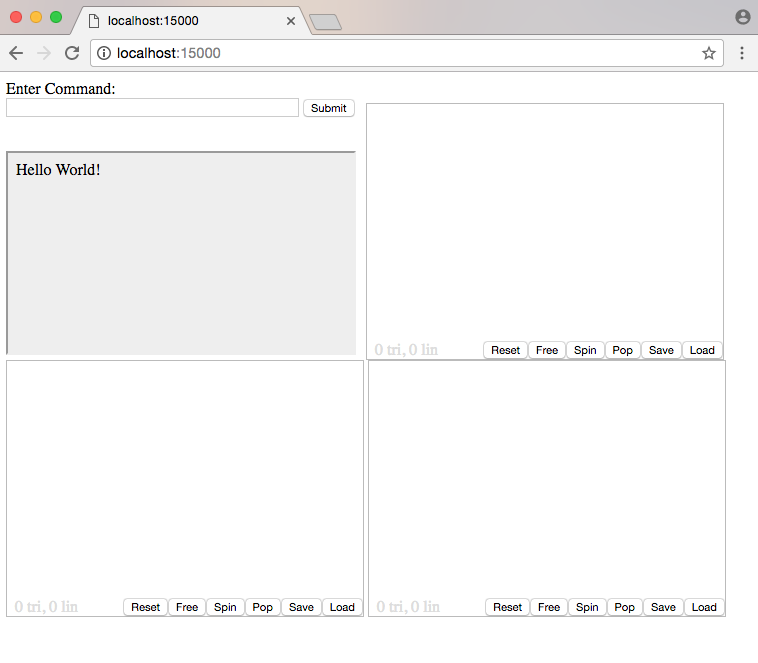
\includegraphics[width=0.75\textwidth]{pix/helloworld.png}
\caption{\f{WEBGUI} after calling \textbf{webwriteline}("Hello World!").}
\label{fig:2}
\end{figure}
\begin{verbatim}
#include <webgui.h>
#include <string.h>
#include <unistd.h>

int main(){
    char str[80];
    strcpy(str,"Hello World!");
    webstart(15000);
    webwriteline(str);
    pause();
    return 0;
}
\end{verbatim}

%%%%%%%%%%%%%%%%%%%%%%%%%%%%%%%%%%%%%%%%%%%%%%%%%%%%%%%%%%%%%%%%%%%%%%%%%%%%
% WEBREADLINE
%%%%%%%%%%%%%%%%%%%%%%%%%%%%%%%%%%%%%%%%%%%%%%%%%%%%%%%%%%%%%%%%%%%%%%%%%%%%
\newpage
\subsection{webreadline}
\label{sec:2-7}
\underline{Description} The function \textbf{void webreadline(char* str)} retrieves the oldest unread string from the
command string queue. If no strings are available, this function call will wait and not return until it receives
a string. Whenever the user submits a command string from the web browser, that string is placed in the command string
queue. If the web browser has buttons showing, pushing the buttons generates a command string as described
in Section \ref{sec:3-3} and places that command string in the queue.\\
\\
\underline{Declaration}
\begin{verbatim} 
	void webreadline(char* str)
\end{verbatim}
\underline{Parameters} \textbf{str} is a char buffer of length 80. After calling \textbf{webreadline}, this buffer
will contain the oldest unread command string. The returned string will not be null terminated as is the convenction
of C strings. Instead the unused portion of the buffer will be filled with the space character as is the convenction of
Fortran strings.\\
\\
\underline{Example} The following example shows the usage of \textbf{webreadline}.
\begin{verbatim}
#include <webgui.h>
#include <stdio.h>

int main(){
    char str[80];
    webstart(15000);
    while(1){
        webreadline(str);
        printf("%.80s\n",str);
    }
    return 0;
}
\end{verbatim}
After compiling and running the above program, the standard output will display any command string(s) that are
submitted by the user in the web browser interface.

%%%%%%%%%%%%%%%%%%%%%%%%%%%%%%%%%%%%%%%%%%%%%%%%%%%%%%%%%%%%%%%%%%%%%%%%%%%%
% WEBINIT
%%%%%%%%%%%%%%%%%%%%%%%%%%%%%%%%%%%%%%%%%%%%%%%%%%%%%%%%%%%%%%%%%%%%%%%%%%%%
\newpage
\subsection{webinit}
\label{sec:2-1}
\underline{Description} The function \textbf{void webinit(char* str, int len)} is called before \textbf{webstart}
if the user wishes to have command buttons on their web browser GUI. Pushing these buttons generates command strings
similar to typing commands when buttons are not present. Additionally, the web browser GUI can store parameter
values associated with your program and allow the user to view and change them. See Section \ref{sec:3-2} for more info.\\
\\
\underline{Declaration}
\begin{verbatim} 
	void webinit(char* str, int len)
\end{verbatim}
\underline{Parameters}\\
\textbf{str} is an array of strings where each string is length 80. These strings can be
either null terminated as is the convention of C strings or they can be padded with spaces as is the convenction
of Fortran strings. However, the second string must start at str[80], and the third string at str[160], etc. A
description on how to format \textbf{str} to create buttons and define parameters can be found in Section \ref{sec:3-2}.\\
\textbf{len} is a (4 byte) integer stating how many strings are present in the array.\\
\\
\underline{Example} The following example shows the usage of \textbf{webinit}.
\begin{verbatim}
#include <webgui.h>
#include <unistd.h>

int main(){
    char str[14][80] = {
        "c c=BuildTire, k=t",
        "c c=BuildEngine, k=e",
        "c c=AssembleCar, k=c",
        "n n=TireRadius, a=tr, t=r, i=1, d=12.5",
        "n n=TireColor, a=tc, t=s, i=1, d=red",
        "n n=EngineSize, a=es, t=i, i=1, d=300",
        "n n=CarColor, a=cc, t=i, i=2, d=1",
        "r c=BuildTire, n=TireRadius",
        "r c=BuildTire, n=TireColor",
        "r c=BuildEngine, n=EngineSize",
        "r c=AssembleCar, n=CarColor",
        "s n=CarColor, v=0, l=red",
        "s n=CarColor, v=1, l=white",
        "s n=CarColor, v=2, l=blue"
    };
    webinit((char*)str,14);
    webstart(15000);
    pause();
    return 0;
}
\end{verbatim}
After compiling and running the above program, the web browser GUI will have 3 command buttons (labeled BuildTire,
BuildEngine, and AssembleCar) and each button will have a drop down menu to view and change associated parameters.
Furthermore, the parameter CarColor (which is in the drop down menu of AssembleCar) will have its own drop down
menu to help select a value. See Figure \ref{fig:3}. Additionally, 4 parameters will be stored in the web browser GUI
(TireRadius, TireColor, EngineSize, and CarColor). These parameters will be viewable and changeable by the user.
To learn more about creating buttons and defining parameters, see Section \ref{sec:3-2}.
\begin{figure}[b!]
\centering
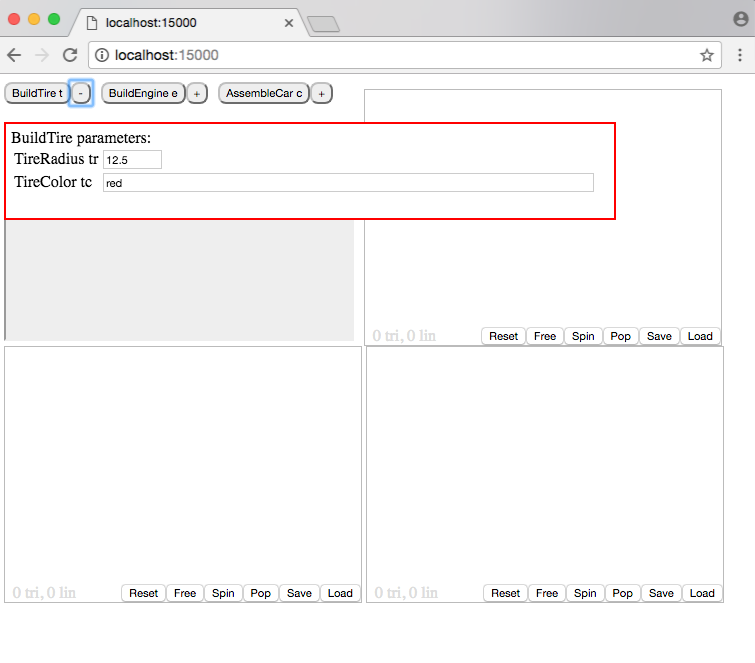
\includegraphics[width=0.75\textwidth]{pix/buttons.png}
\caption{\f{WEBGUI} after calling \textbf{webinit} to create 3 command buttons and store 4 parameters. In this picture,
the user has toggled the drop down menu for BuildTire revealing 2 parameters.}
\label{fig:3}
\end{figure}

%%%%%%%%%%%%%%%%%%%%%%%%%%%%%%%%%%%%%%%%%%%%%%%%%%%%%%%%%%%%%%%%%%%%%%%%%%%%
% WEBUPDATE
%%%%%%%%%%%%%%%%%%%%%%%%%%%%%%%%%%%%%%%%%%%%%%%%%%%%%%%%%%%%%%%%%%%%%%%%%%%%
\newpage
\subsection{webupdate}
\underline{Description} The function \textbf{void webupdate(int* ip, double* rp, char* sp)} updates (changes)
the parameters being stored in the web browser GUI. By default, the web browser GUI doesn't store any parameters,
but by using \textbf{webinit}, you can have the GUI store variables (so the user can view and change them).
The function \textbf{webupdate} can be called anytime after \textbf{webinit} (and before or after \textbf{webstart}). Read
Section \ref{sec:3-4} to learn more about parameters and updating them.\\
\\
\underline{Declaration}
\begin{verbatim} 
	void webupdate(int* ip, double* rp, char* sp)
\end{verbatim}
\underline{Parameters}\\
\textbf{ip} is an array of (4 byte) integers. If your web browser GUI is storing integer parameters (as a result of
a previous call to \textbf{webinit}), they will be updated to these values.\\
\textbf{rp} is an array of (8 byte) doubles. If your web browser GUI is storing double parameters (as a result of
a previous call to \textbf{webinit}), they will be updated to these values.\\
\textbf{sp} is an array of strings of length 80. If your web browser GUI is storing string parameters (as a result of
a previous call to \textbf{webinit}), they will be updated to these values. These strings can be
either null terminated as is the convention of C strings or they can be padded with spaces as is the convenction
of Fortran strings. However, the second string must start at str[80], and the third string at str[160], etc. Therefore,
be careful if you use \textbf{malloc} in C. Make sure to allocate a contiguous block of memory.\\
\\
\underline{Example} The following example shows the usage of \textbf{webupdate}.
\begin{verbatim}
#include <webgui.h>
#include <unistd.h>

int main(){
    char str[14][80] = {
        "c c=BuildTire, k=t",
        "c c=BuildEngine, k=e",
        "c c=AssembleCar, k=c",
        "n n=TireRadius, a=tr, t=r, i=1, d=12.5",
        "n n=TireColor, a=tc, t=s, i=1, d=red",
        "n n=EngineSize, a=es, t=i, i=1, d=300",
        "n n=CarColor, a=cc, t=i, i=2, d=1",
        "r c=BuildTire, n=TireRadius",
        "r c=BuildTire, n=TireColor",
        "r c=BuildEngine, n=EngineSize",
        "r c=AssembleCar, n=CarColor",
        "s n=CarColor, v=0, l=red",
        "s n=CarColor, v=1, l=white",
        "s n=CarColor, v=2, l=blue"
    };
    int ip[2] = {400,2};
    double rp[1] = {13.5};
    char sp[1][80] = {"black"};
    webinit((char*)str,14);
    webstart(15000);
    webupdate(ip,rp,(char*)sp);
    pause();
    return 0;
}
\end{verbatim}
After compiling and running the above program, initially the parameter values of TireRadius, TireColor, EngineSize,
and CarColor are set to 12.5, red, 300, and 1 respectively. The call to \textbf{webupddate} changes these values
to 13.5, black, 400, and 2 respectively.
\begin{figure}[b!]
\centering
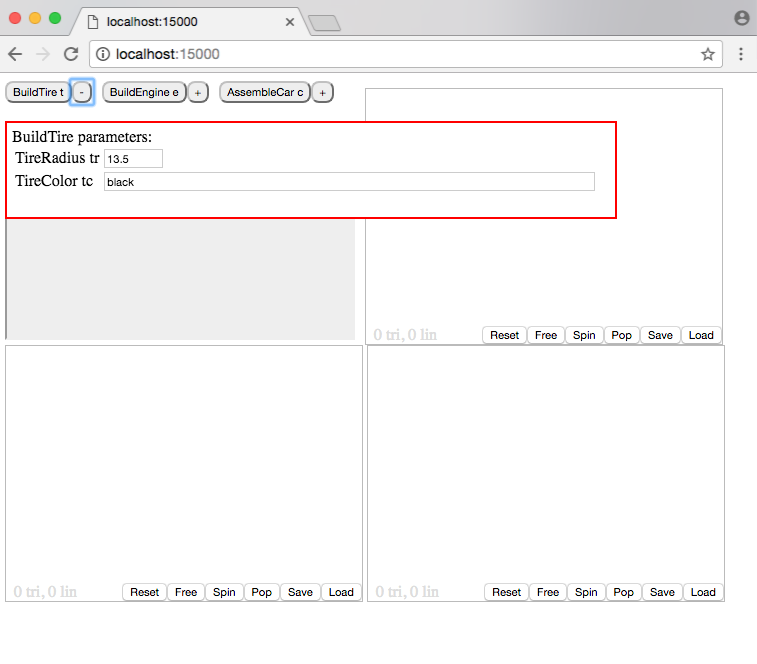
\includegraphics[width=0.75\textwidth]{pix/buttons2.png}
\caption{\f{WEBGUI} after calling \textbf{webinit} and then \textbf{webupdate}. Parameter values TireRadius and TireColor
changed from 12.5 and red to 13.5 and black.}
\label{fig:4}
\end{figure}

%%%%%%%%%%%%%%%%%%%%%%%%%%%%%%%%%%%%%%%%%%%%%%%%%%%%%%%%%%%%%%%%%%%%%%%%%%%%
% WEBSETTITLE
%%%%%%%%%%%%%%%%%%%%%%%%%%%%%%%%%%%%%%%%%%%%%%%%%%%%%%%%%%%%%%%%%%%%%%%%%%%%
\newpage
\subsection{websettitle}
\underline{Description} The function \textbf{void websettitle(char* str)} is called before \textbf{webstart} if the user wishes for the web browser GUI's
webpage to show a title on top of the web browser.\\
\\
\underline{Declaration}
\begin{verbatim} 
	void websettitle(char* str)
\end{verbatim}
\underline{Parameters} \textbf{str} is a string of length 80 or less. This string can either be null terminated as is the convention 
of C strings, or the unused characters of the array length should be filled with spaces as is the convention of Fortran strings.\\
\\
\underline{Example} The following example shows the usage of \textbf{webwriteline}.
\begin{verbatim}
#include <webgui.h>
#include <unistd.h>

int main(){
    websettitle("Sample program");
    webstart(15000);
    pause();
    return 0;
}
\end{verbatim}
After compiling and running the above program, the web browser's webpage will show the title, "Sample program".

%%%%%%%%%%%%%%%%%%%%%%%%%%%%%%%%%%%%%%%%%%%%%%%%%%%%%%%%%%%%%%%%%%%%%%%%%%%%
% WEBSTOP
%%%%%%%%%%%%%%%%%%%%%%%%%%%%%%%%%%%%%%%%%%%%%%%%%%%%%%%%%%%%%%%%%%%%%%%%%%%%
\subsection{webstop}
\underline{Description} The function \textbf{void webstop()} terminates the web server. Afterward web browsers can no longer
connect and display the graphical interface. Also, the listening thread is terminated and all memory is freed.\\
\\
\underline{Declaration} 
\begin{verbatim} 
	void webstop()
\end{verbatim}


\newpage
\section{2D Image display}
\label{sec:2-3}
%%%%%%%%%%%%%%%%%%%%%%%%%%%%%%%%%%%%%%%%%%%%%%%%%%%%%%%%%%%%%%%%%%%%%%%%%%%%
% WEBSETCOLORS
%%%%%%%%%%%%%%%%%%%%%%%%%%%%%%%%%%%%%%%%%%%%%%%%%%%%%%%%%%%%%%%%%%%%%%%%%%%%
\subsection{websetcolors}
\underline{Description} The function \textbf{void websetcolors(int nc, double* R, double* G, double* B, int pane)} 
defines a color palette to be used by subsequent calls. Colors are defined by giving their red, green, blue amounts.
This function defines a color palette for one of the three display panes. Each pane has two palettes; one for 2D images and
one for 3D objects. Call this function before sending any information about
2D images with \textbf{webimagedisplay} and before sending any information about 3D objects with \textbf{webline} and
\textbf{webfill}.\\
\\
\underline{Declaration} 
\begin{verbatim} 
    void websetcolors(int nc, double* R, double* G, double* B, int pane)
\end{verbatim}
\underline{Parameters} \textbf{nc} is a (4 byte) integer stating the number of colors in the palette. 
For 2D images, the maximum value of \textbf{nc} is 256. (For 3D objects, max is 2 billion.)\\
\textbf{R} is an array of (8 byte) doubles. The length of the array is \textbf{nc}. The first element of this array
is the amount of red in the first color. The value of each element should be between 0.0 and 1.0 inclusive.\\
\textbf{G} is an array of (8 byte) doubles. The length of the array is \textbf{nc}. The first element of this array
is the amount of green in the first color.  The value of each element should be between 0.0 and 1.0 inclusive.\\
\textbf{B} is an array of (8 byte) doubles. The length of the array is \textbf{nc}. The first element of this array
is the amount of blue in the first color.  The value of each element should be between 0.0 and 1.0 inclusive.\\
\textbf{pane} is a (4 byte) integer stating which display pane's color palette you are defining. Use integers
0, 1, 2 to define palettes for 3D objects corresponding with panes top right, bottom left, and bottom right respectively. 
Use 3, 4, 5 to define the color palette's for 2D images corresponding with panes top right, bottom left, and bottom 
right respectively.\\
\\
\underline{Example} The following example shows the usage of \textbf{websetcolors}. Imagine that you would like
to define and later use the 6 colors of the rainbow. In conventional RGB, red is RGB = (255,0,0); orange is 
RGB = (255,128,0); yellow is RGB = (255,255,0); green is RGB = (0,255,0); blue is RGB = (0,0,255); and purple
is RGB = (128,0,128). The follow code defines this palette for a 2D image in pane 3.
\begin{verbatim}
double red[6] = {1.0, 1.0, 1.0, 0.0, 0.0, 0.5};
double green[6] = {0.0, 0.5, 1.0, 1.0, 0.0, 0.0};
double blue[6] = {0.0, 0.0, 0.0, 0.0, 1.0, 0.5};
websetcolors(6,red,green,blue,3); 
\end{verbatim}
This program defines a color palette with the 6 colors of the rainbow for 2D images in pane 3. Subsequent calls to 
\textbf{webimagedisplay} in the top right display pane will use this color palette.

%%%%%%%%%%%%%%%%%%%%%%%%%%%%%%%%%%%%%%%%%%%%%%%%%%%%%%%%%%%%%%%%%%%%%%%%%%%%
% WEBIMAGEDISPLAY
%%%%%%%%%%%%%%%%%%%%%%%%%%%%%%%%%%%%%%%%%%%%%%%%%%%%%%%%%%%%%%%%%%%%%%%%%%%%
\newpage
\subsection{webimagedisplay}
\underline{Description} The function \textbf{void webimagedisplay(int nx, int ny, int* image, int pane)} displays a
2D image in the designated display pane. Before calling this, you must call \textbf{websetcolors} to define a palette
to be referenced.\\
\\
\underline{Declaration}
\begin{verbatim}
void webimagedisplay(int nx, int ny, int* image, int pane)
\end{verbatim}
\underline{Parameters} \textbf{nx} is a (4 byte) integer stating the pixel width of the image to be displayed. The
variable \textbf{nx} must be divisible by 4.\\
\textbf{ny} is a (4 byte) integer stating the pixel height of the image to be displayed.\\
\textbf{image} is an array of (4 byte) integers of size \textbf{nx} width and \textbf{ny} height. Each integer represents
a pixel. Each integer's value is between and including 0 and \textbf{nc}-1, the number of colors in the palette you previously 
declared by calling \textbf{websetcolors}. Note that the first color in your palette is referred to as 0 not 1. The second 
color is 1, not 2, etc. The variable \textbf{image} is assumed to reside in memory contiguously row by row as is the 
convention in C. Fortran stores arrays column by column so you need to be careful. Furthermore, the image is drawn 
row by row from the bottom upward.  So your array's first row of integers 
will be the bottom row of your image and your array's last row of integers will be the top row of your image. 
Also note that your image will display in a rectangle with aspect ratio 1.5 width by 1.0 height. (Therefore it looks best
if $nx = 1.5 ny$. This is optional not mandatory.) See example below.\\
\textbf{pane} is a (4 byte) integer stating which display pane to display the image in. Valid integers are 3, 4, 5. These
refer to the top right, bottom left, and bottom right display panes respectively. Note that this integer should match the 
integer that you used to set the palette with \textbf{websetcolors}. \\
\\
\underline{Example} The following example shows the usage of \textbf{webimagedisplay} in the C programming language.
\begin{verbatim}
double red[7] = {1.0, 1.0, 1.0, 0.0, 0.0, 0.5, 0.0};
double green[7] = {0.0, 0.5, 1.0, 1.0, 0.0, 0.0, 0.0};
double blue[7] = {0.0, 0.0, 0.0, 0.0, 1.0, 0.5, 0.0};
websetcolors(7,red,green,blue,3); 
int image[6][4] = { 
    {0,0,0,6},
    {1,1,1,6}, 
    {2,2,2,6}, 
    {3,3,3,6}, 
    {4,4,4,6},
    {5,5,5,6}
};
webimagedisplay(4,6,image,3);
\end{verbatim}
After this program is compiled and ran, it will display an image in the top right display pane as show in Figure \ref{fig:5}.
The first call to \textbf{websetcolors} defines a 2D image palette in pane 3 with colors 0, 1, 2, 3, 4, 5, 6 being red, orange, yellow, green, 
blue, purple, black respectively. The second call to \textbf{webimagedisplay} defines and draws the image.
Notice how the first row of "0,0,0,6" which refers to colors red, red, red, black is the bottom row of the image and the last
row "5,5,5,6" which refers to colors purple, purple, purple, black is the first row of the image. This is illustrated in Figure \ref{fig:6}.

Note that Fortran places arrays of integers in memory contiguously column by column. Therefore to display this same image 
in Fortran, the code would be:

\begin{verbatim}
integer(kind=4), dimension(4,6) :: image
real(kind=8), dimension(7) :: red,green,blue
data r/1.0,1.0,1.0,0.0,0.0,0.5,0.0/
data g/0.0,0.5,1.0,1.0,0.0,0.0,0.0/
data b/0.0,0.0,0.0,0.0,1.0,0.5,0.0/
do j=1,6
    do i=1,3
        image(i,j)=j-1
    enddo
    image(4,j)=6
enddo
call websetcolors(7,red,green,blue,3)
call webimagedisplay(4,6,image,3)
\end{verbatim}

or you could force Fortran to place rows together in memory by writing this:

\begin{verbatim}
integer(kind=4), dimension(24) :: image
do i=0,5
    do j=1,3
        image(4*i+j)=i
    enddo
    image(4*i+4)=6
enddo
call websetcolors(7,red,green,blue,3)
call webimagedisplay(4,6,image,3)
\end{verbatim}

Another example of using \textbf{webimagedisplay} can be found in Section \ref{sec:2-11}. See example 2.

\newpage
\begin{figure}[H]
\centering
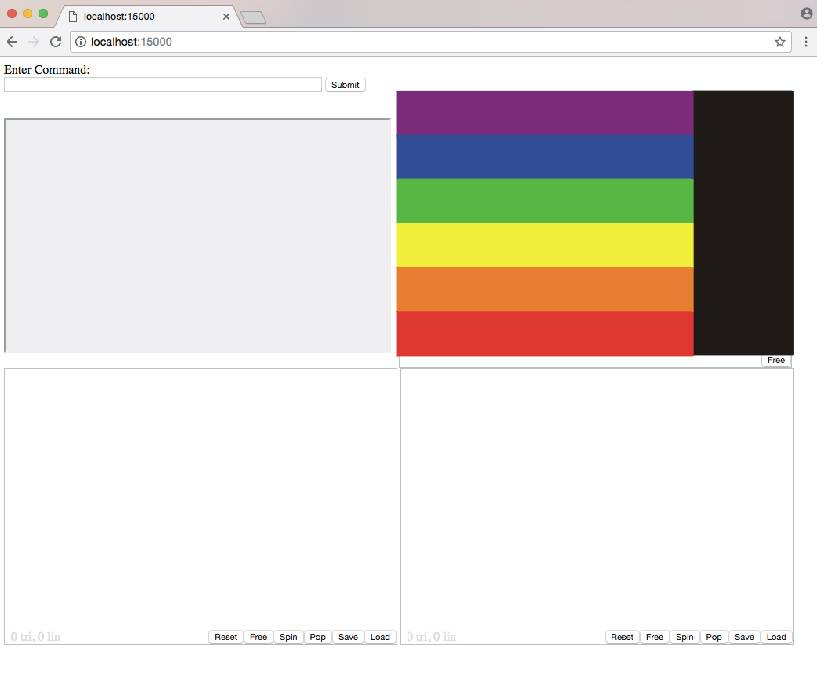
\includegraphics[width=0.75\textwidth]{pix/image2.jpg}
\caption{\f{WEBGUI} after calling \textbf{websetcolors} and \textbf{webimagedisplay}.}
\label{fig:5}
\end{figure} 

\begin{figure}[H]
\centering
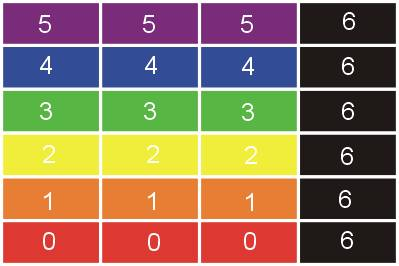
\includegraphics[width=0.75\textwidth]{pix/image3.jpg}
\caption{How the \textbf{image} array becomes an image.}
\label{fig:6}
\end{figure}
 
\newpage
\section{3D Object display}
\label{sec:2-4}
%%%%%%%%%%%%%%%%%%%%%%%%%%%%%%%%%%%%%%%%%%%%%%%%%%%%%%%%%%%%%%%%%%%%%%%%%%%%
% WEBSETCOLORS
%%%%%%%%%%%%%%%%%%%%%%%%%%%%%%%%%%%%%%%%%%%%%%%%%%%%%%%%%%%%%%%%%%%%%%%%%%%%
\subsection{websetcolors}
\underline{Description} The function \textbf{void websetcolors(int nc, double* R, double* G, double* B, int pane)} 
defines a color palette to be used by subsequent calls. Colors are defined by giving their red, green, blue amounts.
This function defines a color palette for one of the three display panes. Each pane has two palettes; one for 2D images and
one for 3D objects. Call this function before sending any information about
2D images with \textbf{webimagedisplay} and before sending any information about 3D objects with \textbf{webline} and
\textbf{webfill}.\\
\\
\underline{Declaration} 
\begin{verbatim} 
    void websetcolors(int nc, double* R, double* G, double* B, int pane)
\end{verbatim}
\underline{Parameters} \textbf{nc} is a (4 byte) integer stating the number of colors in the palette.\\
\textbf{R} is an array of (8 byte) doubles. The length of the array is \textbf{nc}. The first element of this array
is the amount of red in the first color. The value of each element should be between 0.0 and 1.0 inclusive.\\
\textbf{G} is an array of (8 byte) doubles. The length of the array is \textbf{nc}. The first element of this array
is the amount of green in the first color.  The value of each element should be between 0.0 and 1.0 inclusive.\\
\textbf{B} is an array of (8 byte) doubles. The length of the array is \textbf{nc}. The first element of this array
is the amount of blue in the first color.  The value of each element should be between 0.0 and 1.0 inclusive.\\
\textbf{pane} is a (4 byte) integer stating which display pane's color palette you are defining. Use integers
0, 1, 2 to define palettes for 3D objects corresponding with panes top right, bottom left, and bottom right respectively. 
Use 3, 4, 5 to define the color palette's for 2D images corresponding with panes top right, bottom left, and bottom 
right respectively.\\
\\
\underline{Example} The following example shows the usage of \textbf{websetcolors}. Imagine that you would like
to define and later use the 6 colors of the rainbow. In conventional RGB, red is RGB = (255,0,0); orange is 
RGB = (255,128,0); yellow is RGB = (255,255,0); green is RGB = (0,255,0); blue is RGB = (0,0,255); and purple
is RGB = (128,0,128). The follow code defines this palette for a 2D image in pane 3.
\begin{verbatim}
double red[6] = {1.0, 1.0, 1.0, 0.0, 0.0, 0.5};
double green[6] = {0.0, 0.5, 1.0, 1.0, 0.0, 0.0};
double blue[6] = {0.0, 0.0, 0.0, 0.0, 1.0, 0.5};
websetcolors(6,red,green,blue,3); 
\end{verbatim}
This program defines a color palette with the 6 colors of the rainbow for 2D images in pane 3. Subsequent calls to 
\textbf{webimagedisplay} in the top right display pane will use this color palette.

%%%%%%%%%%%%%%%%%%%%%%%%%%%%%%%%%%%%%%%%%%%%%%%%%%%%%%%%%%%%%%%%%%%%%%%%%%%%
% WEBFRAME
%%%%%%%%%%%%%%%%%%%%%%%%%%%%%%%%%%%%%%%%%%%%%%%%%%%%%%%%%%%%%%%%%%%%%%%%%%%%
\newpage
\subsection{webframe}
\label{sec:2-12}
\underline{Description} The function \textbf{void webframe(int frame)} declares which portion of a display pane subsequent 
calls to \textbf{webline} and \textbf{webfill} will draw in. The web browser GUI has 3 display panes and each display pane is divided
into 3 frames (or sub panes). Call this function after \textbf{websetcolors} and before drawing lines and polygons with \textbf{webline} 
and \textbf{webfill}. Note that to draw multiple lines and polygons in a particular frame, you only need to call \textbf{webframe} once and 
then follow with multiple calls to \textbf{webline} and \textbf{webfill}.\\
\\
\underline{Declaration}
\begin{verbatim}
void webframe(int frame)
\end{verbatim}
\underline{Parameters} \textbf{frame} is a (4 byte) integer stating which frame to draw future calls to \textbf{webline} and \textbf{webfill} in.
Valid integers are 1, 2, 3, 4, 5. Each display pane is a rectangle with aspect ratio width to height as 1.5 to 1.0. This rectangle is the 
union of 3 squares, see Figure \ref{fig:10}. The big square on the left is $frame = 4$, the square in the top right is $frame = 2$, and the square
in the bottom right is $frame = 3$. After declaring a frame, all subsequent calls will draw in this square only. After drawing to frames 2, 3, 4,
the resultant 3D objects will not be able to be zoomed, panned, nor rotated. If you wish for your object to be zoomed, panned, and rotated
then draw to $frame = 5$. Frame 5 draws to the big square on the left ($frame=4$) but provides the ability of zoom, pan, and rotate. Lastly,
set $frame=1$ if you wish to draw to the entire rectangle display pane ignoring the sub pane structure.\\
\\
\underline{Example} To see an example of \textbf{webframe}, read the example in the next subsection \ref{sec:2-5}, \textbf{webline}.

\begin{figure}[H]
\centering
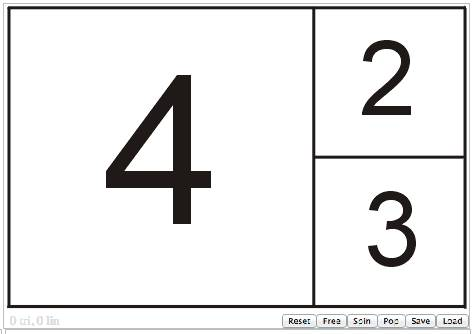
\includegraphics[width=0.75\textwidth]{pix/frame.jpg}
\caption{Frames 2, 3, 4 within a display pane.}
\label{fig:10}
\end{figure} 

%%%%%%%%%%%%%%%%%%%%%%%%%%%%%%%%%%%%%%%%%%%%%%%%%%%%%%%%%%%%%%%%%%%%%%%%%%%%
% WEBLINEFLT
%%%%%%%%%%%%%%%%%%%%%%%%%%%%%%%%%%%%%%%%%%%%%%%%%%%%%%%%%%%%%%%%%%%%%%%%%%%%
\newpage
\subsection{weblineflt}
\label{sec:2-5}
\underline{Description} The function \textbf{void weblineflt(float* x, float* y, float* z, int n, int color)} draws a line in the display pane
that was last declared with \textbf{websetcolors} using the colors declared in \textbf{websetcolors} and within the sub pane (frame)
declared with the last call to \textbf{webframe}.\\
\\
\underline{Declaration}
\begin{verbatim}
void weblineflt(float* x, float* y, float* z, int n, int color)
\end{verbatim}
\underline{Parameters} \textbf{x, y, z} are arrays of (4 byte) single precision floating point real numbers. The first number in each array
are the $x,y,z$ coordinates of your first point in 3D. The second elements are the second point, etc. You can submit any number of points 
and this function draws line segments between each consecutive pair of points. The values of \textbf{x,y,z} are between 0.0 and 1.0 inclusive.
The center of each frame (sub pane) is $(x,y,z)=(0.5,0.5,0.5)$, the bottom left corner is $(x,y,z)=(0,0,z)$ and the top right corner is $(x,y,z)=(1,1,z)$.
Positive \textbf{z} comes out of the screen, while negative \textbf{z} goes into the screen.
An exception to these bounds is $frame = 1$ which accesses the entire display pane rectangle. 
In this case the value of \textbf{x} is between 0.0 and 1.5 inclusive. (and \textbf{y} is still between 0.0 and 1.0). The 
bottom left corner is $(x,y,z)=(0,0,z)$ and the top right corner is $(x,y,z)=(1.5,1,z)$.\\
\textbf{n} is a (4 byte) integer stating the length of arrays \textbf{x,y,z} which is the number of 3D points that your are submitting.\\
\textbf{color} is a (4 byte) integer between 1 and \textbf{nc}, where \textbf{nc} is the number of colors you declared in your last call
to \textbf{websetcolors}. The value \textbf{color} references those colors with 1 being the first color (not 0), 2 the second (not 1), etc. 
All line segments will be drawn with this color.\\
\\
\underline{Example} The following example shows the usage of \textbf{weblineflt}.
\begin{verbatim}
double red[3]={1.0,0.0,0.0};
double green[3]={0.0,1.0,0.0};
double blue[3]={0.0,0.0,1.0};
websetcolors(3,red,green,blue,0);
float x[4]={0.0,0.75,0.5,0.0};
float y[4]={0.0,0.25,0.75,0.0};
float z[4]={0.5,0.5,0.5,0.0};
webframe(4);
weblineflt(x,y,z,4,1);
webframe(3);
weblineflt(x,y,z,4,2);
webframe(2);
weblineflt(x,y,z,4,3);
webgldisplay(0);
\end{verbatim}
The above block of code, defines a 3D object color palette for display pane 0 (top right pane) declaring the 3 colors red, green, blue as a result of the first call to 
\textbf{websetcolors}. Furthermore, \textbf{websetcolors} declares that subsequent calls to \textbf{webline} and \textbf{webfill} will draw lines and polygons 
in display pane 0. The first call to \textbf{webframe} declares future drawing to be in the sub pane of $frame=4$. The subsequent call to \textbf{weblineflt} draws a 
triangle of $color=1$ which is red into $frame=4$ of $pane=0$. A second call to \textbf{webframe} and \textbf{weblineflt} draws a triangle of  $color=2$ 
which is green into $frame=2$ of $pane=0$. And a third call to  \textbf{webframe} and \textbf{weblineflt} draws a triangle of $color=3$ which is blue into 
$frame=3$ of $pane=0$. Lastly, calling \textbf{webgldisplay} displays the 3D object in display pane 0. See Figure \ref{fig:8}.

\begin{figure}[H]
\centering
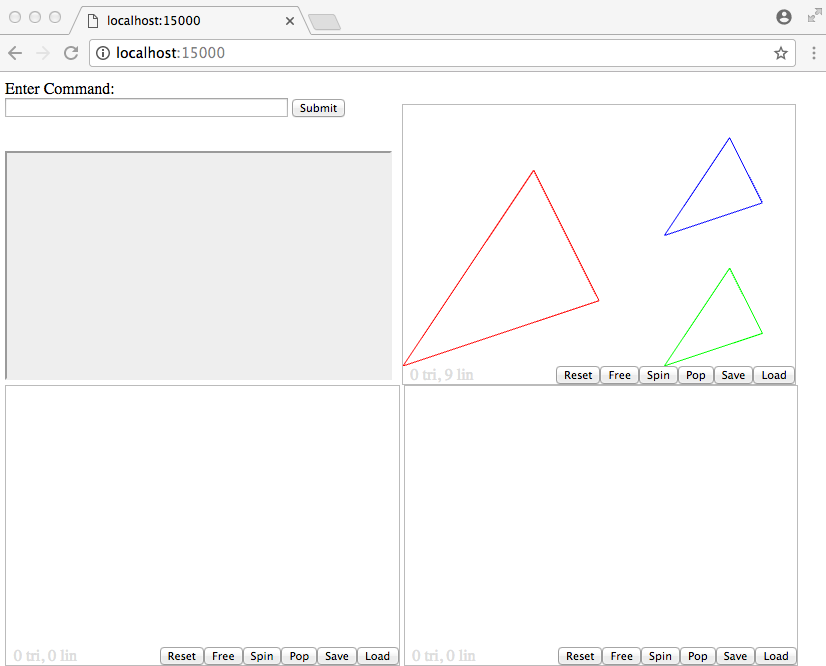
\includegraphics[width=0.75\textwidth]{pix/lines.png}
\caption{\f{WEBGUI} after calling \textbf{webline} three times in display pane 0 with different frames and colors.}
\label{fig:8}
\end{figure} 

Below is another example. It draws a black triangle in $frame=1$ of $pane=1$. Output shown in Figure \ref{fig:9}.
\begin{verbatim}
double red[1]={0.0};
double green[1]={0.0};
double blue[1]={0.0};
websetcolors(1,red,green,blue,1);
float x[4]={0.0,1.5,0.25,0.0};
float y[4]={0.75,0.25,0.25,0.75};
float z[4]={0.5,0.5,0.5,0.5};
webframe(1);
weblineflt(x,y,z,4,1);
webgldisplay(1);
\end{verbatim}
\begin{figure}[H]
\centering
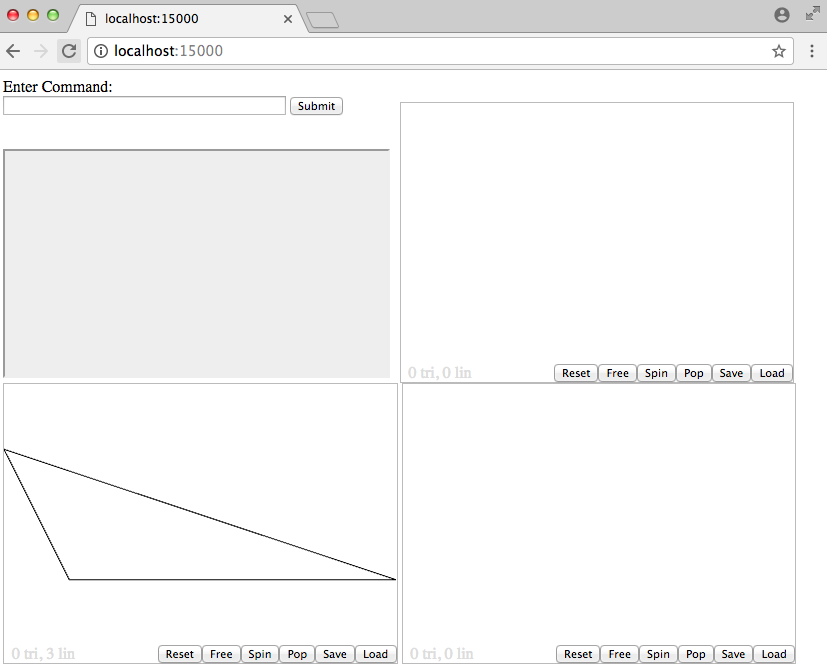
\includegraphics[width=0.75\textwidth]{pix/lines2.png}
\caption{\f{WEBGUI} after calling \textbf{webframe(1)} and \textbf{webline} in display pane 1.}
\label{fig:9}
\end{figure}

%%%%%%%%%%%%%%%%%%%%%%%%%%%%%%%%%%%%%%%%%%%%%%%%%%%%%%%%%%%%%%%%%%%%%%%%%%%%
% WEBFILLFLT
%%%%%%%%%%%%%%%%%%%%%%%%%%%%%%%%%%%%%%%%%%%%%%%%%%%%%%%%%%%%%%%%%%%%%%%%%%%%
\newpage
\subsection{webfillflt}
\label{sec:2-6}
\underline{Description} The function \textbf{void webfillflt(float* x, float* y, float* z, int n, int color)} draws a filled convex polygon in the display pane
that was last declared with \textbf{websetcolors} using the colors declared in \textbf{websetcolors} and within the sub pane (frame)
declared with the last call to \textbf{webframe}.\\
\\
\underline{Declaration}
\begin{verbatim}
void webfillflt(float* x, float* y, float* z, int n, int color)
\end{verbatim}
\underline{Parameters} \textbf{x, y, z} are arrays of (4 byte) single precision floating point real numbers. The first number in each array
are the $x,y,z$ coordinates of your first vertex in 3D. The second elements are the second vertex, etc. You can submit any number of vertices 
and this function draws filled triangles between each consecutive pair of vertices together with the first vertex (thus drawing the entire filled convex polygon). 
The values of \textbf{x,y,z} are between 0.0 and 1.0 inclusive.
The center of each frame (sub pane) is $(x,y,z)=(0.5,0.5,0.5)$, the bottom left corner is $(x,y,z)=(0,0,z)$ and the top right corner is $(x,y,z)=(1,1,z)$.
Positive \textbf{z} comes out of the screen, while negative \textbf{z} goes into the screen.
An exception to these bounds is $frame = 1$ which accesses the entire display pane rectangle. 
In this case the value of \textbf{x} is between 0.0 and 1.5 inclusive. (and \textbf{y} is still between 0.0 and 1.0). The 
bottom left corner is $(x,y,z)=(0,0,z)$ and the top right corner is $(x,y,z)=(1.5,1,z)$.\\
\textbf{n} is a (4 byte) integer stating the length of arrays \textbf{x,y,z} which is the number of 3D vertices that your are submitting.\\
\textbf{color} is a (4 byte) integer between 1 and \textbf{nc}, where \textbf{nc} is the number of colors you declared in your last call
to \textbf{websetcolors}. The value \textbf{color} references those colors with 1 being the first color (not 0), 2 the second (not 1), etc. 
The entire filled polygon (all separate triangles) will be drawn with this color.\\
\\
\underline{Example} The following example shows the usage of \textbf{webfillflt}.
\begin{verbatim}
double red[3] = {1.0, 1.0, 1.0};
double green[3] = {0.0, 0.5, 1.0};
double blue[3] = {0.0, 0.0, 0.0};
websetcolors(3,red,green,blue,0);
webframe(5);
float xA[5]={0.25,0.75,0.75,0.25,0.25};
float yA[5]={0.25,0.25,0.75,0.75,0.25};
float zA[5]={0.75,0.75,0.75,0.75,0.75};
webfillflt(xA,yA,zA,5,1);
float xB[5]={0.25,0.75,0.75,0.25,0.25};
float yB[5]={0.25,0.25,0.25,0.25,0.25};
float zB[5]={0.25,0.25,0.75,0.75,0.25};
webfillflt(xB,yB,zB,5,2);
float xC[5]={0.25,0.25,0.25,0.25,0.25};
float yC[5]={0.25,0.75,0.75,0.25,0.25};
float zC[5]={0.25,0.25,0.75,0.75,0.25};
webfillflt(xC,yC,zC,5,3);
webgldisplay(0);
\end{verbatim}
The above block of code, defines a 3D object color palette for display pane 0 (top right pane) declaring the 3 colors red, orange, yellow as a result of the first call to 
\textbf{websetcolors}. Furthermore, \textbf{websetcolors} declares that subsequent calls to \textbf{webline} and \textbf{webfill} will draw lines and polygons 
in display pane 0. Then \textbf{webframe} declares future drawing to be in the sub pane of $frame=5$. The subsequent call to \textbf{webfillflt} draws one
face of a cube (a square) with $color=1$ which is red into $frame=5$ of $pane=0$. A second call to \textbf{webframe} and \textbf{webfillflt} draws a second face of a cube
with $color=2$ which is orange into $frame=5$ of $pane=0$. And a third call to  \textbf{webframe} and \textbf{webfillflt} draws a third face of a cube with $color=3$ 
which is yellow into $frame=5$ of $pane=0$. Lastly, calling \textbf{webgldisplay} displays the 3D object in display pane 0. After the 3D object is displayed,
the user can rotate the cube so that one vertex is pointed forward. See Figure \ref{fig:11}.
\begin{figure}[H]
\centering
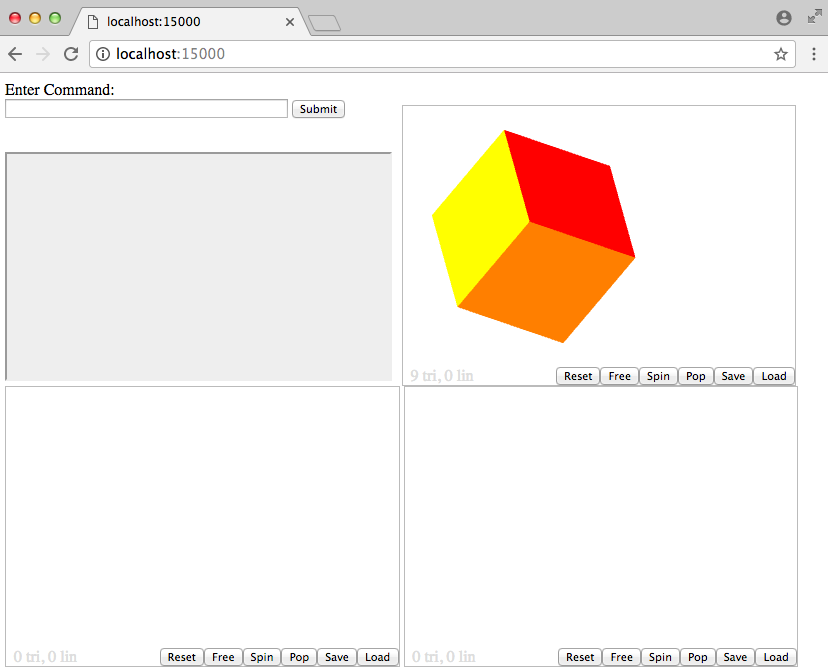
\includegraphics[width=0.75\textwidth]{pix/cube.png}
\caption{\f{WEBGUI} after calling \textbf{webfill} three times in display pane 0 and rotating the object.}
\label{fig:11}
\end{figure} 

%%%%%%%%%%%%%%%%%%%%%%%%%%%%%%%%%%%%%%%%%%%%%%%%%%%%%%%%%%%%%%%%%%%%%%%%%%%%
% WEBLINEDBL and FILLDBL
%%%%%%%%%%%%%%%%%%%%%%%%%%%%%%%%%%%%%%%%%%%%%%%%%%%%%%%%%%%%%%%%%%%%%%%%%%%%
\newpage
\subsection{weblinedbl}
\underline{Description} The function \textbf{void weblinedbl(double* x, double* y, double* z, int n, int color)} is the same as \textbf{weblineflt} 
except that the array arguments are double precision reals instead of single precision. Note that \f{WEBGUI} only draws lines in single 
precision, but you should call either \textbf{weblineflt} or \textbf{weblinedbl} based on how your vertices are stored in your software either as single 
precision (4 byte reals) or double precision (8 byte reals). Don't cast your variables, let \f{WEBGUI} do the casting for you.\\
\\
\subsection{webfilldbl}
\underline{Description} The function \textbf{void webfilldbl(double* x, double* y, double* z, int n, int color)} is the same as \textbf{webfillflt} 
except that the array arguments are double precision reals instead of single precision. Note that \f{WEBGUI} only draws triangles in single 
precision, but you should call either \textbf{weblineflt} or \textbf{weblinedbl} based on how your vertices are stored in your software either as single 
precision (4 byte reals) or double precision (8 byte reals). Don't cast your variables, let \f{WEBGUI} do the casting for you.\\
\\
\subsection{webgldisplay}
\underline{Description} The function \textbf{void webgldisplay(int pane)} displays the 3D object that was previously sent to the indicated display 
pane. Call this function after calling \textbf{websetcolors}, \textbf{webframe}, \textbf{webline}, and \textbf{webfill}.\\
\\
\underline{Declaration}
\begin{verbatim}
void webgldisplay(int pane)
\end{verbatim}
\underline{Parameters} \textbf{pane} is a (4 byte) integer stating which display pane should display its 3D object. Valid integers are 0, 1, 2 
referring to the top right, bottom left, and bottom right display pane. The variable \textbf{pane} should match the value in your previous call
to \textbf{websetcolors}.\\
\\
\underline{Example} For an example of \textbf{webgldisplay}, see the examples in the previous sub sections, \ref{sec:2-5} and \ref{sec:2-6}.

\newpage
\section{Miscellaneous}

%%%%%%%%%%%%%%%%%%%%%%%%%%%%%%%%%%%%%%%%%%%%%%%%%%%%%%%%%%%%%%%%%%%%%%%%%%%%
% WEBQUERY
%%%%%%%%%%%%%%%%%%%%%%%%%%%%%%%%%%%%%%%%%%%%%%%%%%%%%%%%%%%%%%%%%%%%%%%%%%%%
\subsection{webquery}
\underline{Description} The function \textbf{int webquery()} informs the caller whether the web browser is displaying command buttons or not. Even 
if your software calls \textbf{webinit} to create command buttons, the user can toggle them off and on with key strokes, therefore this function exists. 
(To learn how to toggle buttons off and on, see Section \ref{sec:4-1})\\
\\
\underline{Declaration}
\begin{verbatim}
int webquery()
\end{verbatim}
\underline{Return Value} If command buttons are showing, 1 is returned. If a command prompt to accept only typed strings is showing, 0 is returned.
\\
%%%%%%%%%%%%%%%%%%%%%%%%%%%%%%%%%%%%%%%%%%%%%%%%%%%%%%%%%%%%%%%%%%%%%%%%%%%%
% WEBBUTTON
%%%%%%%%%%%%%%%%%%%%%%%%%%%%%%%%%%%%%%%%%%%%%%%%%%%%%%%%%%%%%%%%%%%%%%%%%%%%
\subsection{webbutton}
\underline{Description} The function \textbf{void webbutton(int highlight, char* cmd)} will highlight a command button by making it a darker gray. This
is a useful function to indicate whether a feature of your software is turned on or off.\\
\\
\underline{Declaration}
\begin{verbatim}
void webbutton(int highlight, char* cmd)
\end{verbatim}
\underline{Parameters} \textbf{highlight} is a (4 byte) integer of value 1 or 0. Setting $highlight=1$, causes the indicated command button to be 
highlighted. Setting $highlight=0$ causes the indicated command button to be unhighlighted (normal).\\
\textbf{cmd} is a string of length 20 or less. \textbf{cmd} can be either a NULL terminated C type string, or it can be a Fortran type
string padded with spaces to its array length. The string \textbf{cmd} must match the command name that you supplied in \textbf{webinit} (with
the key value pair associated with c.)\\
\\
%%%%%%%%%%%%%%%%%%%%%%%%%%%%%%%%%%%%%%%%%%%%%%%%%%%%%%%%%%%%%%%%%%%%%%%%%%%%
% WEBPAUSE
%%%%%%%%%%%%%%%%%%%%%%%%%%%%%%%%%%%%%%%%%%%%%%%%%%%%%%%%%%%%%%%%%%%%%%%%%%%%
\subsection{webpause}
\underline{Description} The function \textbf{void webpause()} requests that the user click a continue button before proceeding. This is useful if your 
software is outputting multiple images that potentially overwrite themselves. You can request the user click continue which forces them to view the
image before proceeding.
\\
\underline{Declaration}
\begin{verbatim}
void webpause()
\end{verbatim}

%%%%%%%%%%%%%%%%%%%%%%%%%%%%%%%%%%%%%%%%%%%%%%%%%%%%%%%%%%%%%%%%%%%%%%%%%%%%
% WEBSETMODE
%%%%%%%%%%%%%%%%%%%%%%%%%%%%%%%%%%%%%%%%%%%%%%%%%%%%%%%%%%%%%%%%%%%%%%%%%%%%
\newpage
\subsection{websetmode}
\label{sec:2-11}
\underline{Description} The function \textbf{void websetmode(int x)} can allow your program to receive the keyboard and mouse presses from
the web browser. It can also allow your program to display 2D images or 3D objects faster than the default two per second (thus simulating 
animation). And this function determines whether new 3D objects inherit zoom, pan, and rotation settings from previously displayed 3D objects. 
By default, \f{WEBGUI} runs in mode 0. If this is adequate, you do not need to call \textbf{websetmode}. 
This function can be called as often as you like and before or after \textbf{webstart}. Recommended usage is to change the mode when needed 
and change back to 0 when not needed.\\
\\
\underline{Declaration}
\begin{verbatim}
void websetmode(int x)
\end{verbatim}
\underline{Parameter} \textbf{x} is a (4 byte) integer between -4 and 9 inclusive requesting the desired mode. The fourteen modes are 
listed in the table below.
\begin{center}
\begin{tabular}{|c| c| c| c| c| c|}
\hline
\multicolumn{6}{|c|}{\strutul Valid modes for \textbf{websetmode} } \\
\hline 
\strutul
\textbf{x} & keyboard & mouse & \textbf{webZZZdisplay}  & FPS & reset\\
~ & ~ & ~ & blocking & ~ & position\\
\hline
\strutu
-1 & no & no & no & 2 & no\\
\hline
-2 & yes & no & no & 2 & yes\\
\hline
-3 & no & yes & no & 2 & yes\\
\hline
-4 & yes & yes & no & 2 & yes\\
\hline \hline
0 & no & no & no & 2 & yes\\
\hline
1 & yes & no & no & 2 & no\\
\hline
2 & no & yes & no & 2 & no\\
\hline
3 & yes & yes & no & 2 & no\\
\hline \hline
4 & yes & yes & yes & 10 & no\\
\hline
5 & yes & yes & yes & 20 & no\\
\hline
6 & yes & yes & yes & 30 & no\\
\hline \hline
7 & no & no & yes & 10 & no\\
\hline
8 & no & no & yes & 20 & no\\
\hline
9 & no & no & yes & 30 & no\\
\hline 
\end{tabular}
\end{center}

The second column, keyboard, indicates whether the web browser sends keyboard presses to webgui.c (the server). 
Keyboard presses are sent as command strings. Your program receives the string by calling \textbf{webreadline}. See Section \ref{sec:2-7} 
or Section \ref{sec:3-3}. The string is formatted as follows:
\begin{verbatim}
key code=XXX
\end{verbatim}
where XXX is the key's browser code. To discover browser codes, run \f{WEBGUI} in mode 1, press keys, and read the 
codes from the bottom of the web page. As you press keys in modes -4,-2,1,3,4,5,6, the bottom of the web page says:
\begin{verbatim}
(last pressed key: code = XXX)
\end{verbatim}

The third column, mouse, indicates whether the web browser sends mouse presses to webgui.c. Mouse presses
are sent as command strings. The string is formatted as follows:
\begin{verbatim}
mse button=AAA,x=BBB,y=CCC,pane=DDD
\end{verbatim}
AAA is 0,1,2 referring the the left, center, or right mouse button. (On one button systems, you can simulate the center or right button
by holding the OPTION/ALT key or COMMAND/WINDOWS key on Mac/Windows when you press the left button.) 
BBB is the $x$-coordinate of the mouse click. CCC is the $y$-coordinate
of the mouse click. The $(x,y)$ coordinates are relative to frame=5. (Frames are explained in Section \ref{sec:2-12}).
Clicking in the center of frame=5 sends (0,0), the bottom left corner sends (-1,-1) 
and the top right corner of frame=5 sends (1,1). The reported $(x,y)$ coordinates are the result of mapping the mouse click 
into the $xy$ plane according to the current zoom, pan, and rotation. 
When the display pane contains a 2D image then coordinates are relative to frame=1. 
The bottom left corner sends (0,0) and the top right corner of frame=1 sends (1.5,1). (Pan, zoom, and rotation are not applicable and ignored.)
DDD is 0,1,2 (or 3,4,5 for 2D images) referring to the top right, bottom left, or bottom right display pane. You can view example coordinates 
by running \f{WEBGUI} in mode 2, pressing the mouse button, and reading the bottom of the page which says:
\begin{verbatim}
(last pressed mouse: button = AAA, x = BBB, y = CCC, pane = DDD)
\end{verbatim}

The fourth column, blocking, indicates whether the functions \textbf{webimagedisplay} and
\textbf{webgldisplay} are blocking are not. By default they are not. But in modes 4,5,6,7,8,9 these functions do not return until the web browser
displays the 2D image or 3D object. Thus your program can send 2D images or 3D objects as fast as it can and let \textbf{webZZZdisplay}
regulate the speed of your program.

The fifth column, FPS, indicates the maximum frame rate per second in which the web browser displays
2D images or 3D objects. Note that this rate is how often the web browser polls the server (asks the server if there is a new image or object
to display). Therefore if you don't need a high FPS, then you should choose a lower FPS to minimize bandwidth and socket activity. Also
if your web browser misbehaves, lower the FPS.

The sixth column, reset position, indicates whether sending a new 3D object (WebGL) to a display pane's frame=5 resets the zoom, pan, 
and rotation. By default, in mode=0, when you display a new 3D object, it will display without any zoom, pan, or rotation applied even if you zoomed, 
panned, and rotated the previous 3D object that was in the same display pane. In some situations when the second 3D object
relates to the first 3D object, it is preferable to not reset the zoom, pan, and rotation but instead have the second object inherit the positioning of the
first object.

In addition to controlling "reset position"
by calling \textbf{websetmode}, you can toggle this feature off and on in the web browser by pressing the OPTION + R key. 
(On Windows machines, use ALT instead of OPTION.)

When the web browser is in a mode other than 0, the web browser indicates this by displaying
\begin{verbatim}
INTERACTIVE MODE: YYY
\end{verbatim}
on the bottom of the web page where YYY describes the mode.\\
\\
\underline{Example 1.} The following example shows the usage of \textbf{websetmode}.
\begin{verbatim}
#include <webgui.h>
#include <stdio.h>

int main(){
    char str[80];
    websetmode(3);
    webstart(15000);
    while(1){
        webreadline(str);
        printf("%.80s\n",str);
    }
    return 0;
}
\end{verbatim}
After compiling and running the above program, the web browser will display at the bottom:
\begin{verbatim}
INTERACTIVE MODE: Key and mouse presses sent to server.
\end{verbatim}
And if you hit the "1" key and then click the mouse inside pane 0, the standard output will display:
\begin{verbatim}
key code=49
mse button=0,x=0.473881,y=0.597015,pane=0
\end{verbatim}
\underline{Example 2.} Below is another example which demonstrates animation and keyboard capture. The following code displays 
30 images per second at resolution 720 by 480 pixels (DVD quality):
\begin{verbatim}
#include<stdio.h>
#include<unistd.h>
#include<pthread.h>
#include<webgui.h>

pthread_t pth;
int image[480][720]={{0}};
int x=336, y=216, d=48, v[2]={6,0}, stop=0;
double r[2]={1,1}, g[2]={1,0}, b[2]={1,0};
void *processcommand(void *arg);

int main(){
    int i,j;
    websetmode(6);
    webstart(15000);
    websetcolors(2,r,g,b,3);
    pthread_create(&pth,NULL,processcommand,NULL);
    while(stop==0){
        for (i=0;i<480;i++) for (j=0;j<720;j++) image[i][j]=0;
        for (i=y;i<y+d;i++) for (j=x;j<x+d;j++) image[i%480][j%720]=1;
        webimagedisplay(720,480,(int*)image,3);
        x+=v[0]+720; x%=720;
        y+=v[1]+480; y%=480;
    }
    return 0;
}
void *processcommand(void *arg){
    char str[80];
    while(1){
        webreadline(str);
        if (str[0]=='q') stop=1;
        /* expecting str = "key code=XX" */
        else if (str[0]=='k'){
            if (str[10]=='8') {v[0]=0; v[1]=6;} // up is 38
            if (str[10]=='0') {v[0]=0; v[1]=-6;} // down is 40
            if (str[10]=='7') {v[0]=-6; v[1]=0;} // left is 37
            if (str[10]=='9') {v[0]=6; v[1]=0;} // right is 39
        }
    }
}
\end{verbatim}
After running this program, the web browser will display at the bottom:
\begin{verbatim}
INTERACTIVE MODE: Frame rate = 30 fps. Key and mouse presses sent to server.
\end{verbatim}
and a red square begins to move across display pane 0. Motion is an illusion created by rapidly drawing new images where the 
red square has a different location. Use the arrow keys to change the red square's direction.
The code for this program and another example program which demonstrates drawing dots 
by clicking the mouse are included in the examples folder that came inside the tar file containing this software.

Here's a final remark; the mode should be set within your program by calling \textbf{websetmode}. However for debugging purposes, you can change the
mode during runtime in the web browser. To set a mode, press the OPTION + P key, and then press the OPTION + XXX
where XXX is the number key of the desired mode. On Windows machines use ALT instead of OPTION. To set modes -1,-2,-3,-4, first set the 
mode to 0,1,2,3 and then toggle the "reset position" feature by pressing the OPTION + R key. 

 \newpage
 \cleardoublepage
\setcounter{chapter}{2} %The counter for chapters should be set one less than 
                        %the actual chapter number, for example, {1} for 
                        %chapter 2, and {2} for chapter 3.
\setcounter{section}{3} %The counter for sections should be set to match the
                        %actual chapter number, for example, {2} for sections 
                        %in chapter, and {3} for sections in chapter 3. 
\chapter{GUI Command Buttons and Parameters}
\markboth{WEBGUI USERS' GUIDE}{GUI COMMAND BUTTONS AND PARAMETERS}
\pagenumbering{arabic}
\setcounter{page}{33} %The counter for page numbers must be placed here in your
                     %chapter, following the \chapter and \markboth commands.
                     %It should always be the next available right-hand page.
                     %All chapters start on new rights. It will always be
                     %an odd number.  

 
\section{Introduction}
\label{sec:3-2}
The purpose of a graphical interface is to control some software and display output. Presumably the software 
has a variety of routines (tasks it can perform). And with each routine, there can be associated parameters 
(variables). Therefore, it would be helpful if the GUI can view and change parameters before requesting that a 
routine to be executed. After execution, the GUI should be able to display text and graphical output.

If you only use the command line version of \f{WEBGUI}, you do not need to read this section. If however, you
would like to call \textbf{webinit} to add command buttons and parameter storage in your web browser, then
this section explains how that works.

In order for the web browser interface to provide command buttons and store parameters for viewing and changing,
you must inform the web browser about your software's routines and variables. You accomplish this with the 
\textbf{webinit} call which is described in Section \ref{sec:2-1}.

\section{Calling webinit}
\label{sec:3-1}
The argument of \textbf{webinit} is an array of strings (each 80 characters in length). 
This section describes the formatting of these strings.
There are 4 types of argument strings. Strings that begin with the letter "c" define command buttons. Strings
that begin with the letter "n" define a parameter. Strings that begin with the letter "r" define an association
between a command and a parameter. And strings that begin with the letter "s" define a list of options for
a parameter. All strings have the same format. Each begins with a single letter (either c, n, r, or s) and then each
has a list of key = value pairs separated by commas. Spaces are optional.

Below is the example array of strings we presented in Section \ref{sec:2-1}. These strings create 3 command buttons, 
store 4 parameters (2 integers, 1 real, and 1 string) and provide 3 options for 1 of the parameters. Notice the 4 types 
of strings and the common format. We will explain this example in the 4 sections to follow:
\begin{verbatim}
    char str[14][80] = {
        "c c=BuildTire, k=t",
        "c c=BuildEngine, k=e",
        "c c=AssembleCar, k=c",
        "n n=TireRadius, a=tr, t=r, i=1, d=12.5",
        "n n=TireColor, a=tc, t=s, i=1, d=red",
        "n n=EngineSize, a=es, t=i, i=1, d=300",
        "n n=CarColor, a=cc, t=i, i=2, d=1",
        "r c=BuildTire, n=TireRadius",
        "r c=BuildTire, n=TireColor",
        "r c=BuildEngine, n=EngineSize",
        "r c=AssembleCar, n=CarColor",
        "s n=CarColor, v=0, l=red",
        "s n=CarColor, v=1, l=white",
        "s n=CarColor, v=2, l=blue"
    };
 \end{verbatim}

\subsection{Command buttons}
\label{sec:3-3}
%\begin{table}[htbp]
\begin{center}
\begin{tabular}{|l|l|l|l|}
\hline
\multicolumn{3}{|c|}{\strutul Key-value pairs associated with $c$ string} \\
\hline 
\strutul
Name & Key & Value \\
\hline
\strutu
command button text & c & maximum of 20 characters \\
abbreviation & k & maximum of 3 lowercase characters \\
\hline
\end{tabular}
\end{center}
%\caption{Syntax for $c$ string.}
%\label{table-1}
%\end{table}

Every string that begins with "c" will create a command button in the web browser GUI. The name on the button is the value 
associated with the key c. When this button is pushed, a command string is generated and placed
in the command string buffer. (Your software retrieves this command string when it calls \textbf{webreadline}.)

The format of the generated command string is as follows. The first 1-3 characters will be the abbreviation that you assigned
to that command via the key-value pair of k. The remainder of the command string will be key-value pairs separated by 
commas. The keys will be parameter names that you define with an $n$ string (and associate with an $r$ string) and the 
values will be any parameters that you changed from their defaults with the web browser drop down menus.

For example, if you push the button "Build Tire", the command string transmitted will be an 80 character string with the first letter "e"
and the remaining 79 characters as spaces. If before you push the button "Build Tire", you change the associated parameter
"TireRadius" from its default of 12.5 to 13.5, and "TireColor" from red to while, then the transmitted command string will be 
\begin{verbatim}
e TireRadius=13.5, TireColor=white 
\end{verbatim}
padded out with spaces to length 80.

\subsection{Parameters}
\label{sec:3-4}

\begin{center}
\begin{tabular}{|l|l|l|l|}
\hline
\multicolumn{3}{|c|}{\strutul Key-value pairs associated with $n$ string} \\
\hline 
\strutul
Name & Key & Value \\
\hline
\strutu
parameter name & n & maximum of 20 characters \\
abbreviation & a & maximum of 3 characters \\
data type & t & i (int), r (real), s (string), f (file)\\
\strutl
index & i & pointer to \f{IP}, \f{RP}, \f{SP} \\
default value & d & maximum of 40 characters/digits \\
\hline
\end{tabular}
\end{center}

Every string that begins with "n" will define a parameter for the web browser to store and allow the user to view and change.
When a user changes a parameter via a web browser drop down menu, the new value of that parameter is transmitted
when the associated command button is pressed. (This is described in the subsection prior and following.)

Changed parameter values are also transmitted when you close the drop down menu but have not actually issued the 
associated command. If you close a drop down menu where a parameter has been changed, then a command string
is placed in the command string buffer. This isn't a normal command string. The first 1-3 characters of the command string
are the capital letter version of the associated command abbreviation. It is important that your software is aware of this
and processes these slightly different command strings correctly after receiving them from \textbf{webreadline}. For
example, if you change the parameter "TireRadius" from its default of 12.5 to 13.5, and "TireColor" from red to while, and
then you close the drop down menu (without issuing the "BuildTire" command), then the following command string will be
transmitted:
\begin{verbatim}
E TireRadius=13.5, TireColor=white 
\end{verbatim}
Note that this differs from the command string in the preceding subsection which started with a lowercase "e".

The web browser recognizes 3 types of parameters; integer, real, and string. Strings come in 3 types,  (i) contain
no space characters, (ii) contain space characters, and (iii) file names. If you declare a string as a file name, then the web browser 
will give you a file selection dialog box to change them. Declare a parameter's type by using the key-value pair associated with
t. For a number, set the value to either i or r denoting integer or real respectively. For a string, set the value to either s, l, or f
to denote the string has no spaces, the string has spaces, and file name.  

The web browser also assumes that your software maintains these variables (integers, reals, strings) in 3 arrays, \f{IP}, \f{RP},
\f{SP}. Therefore each parameter that you let the web browser know about needs an index into your software's associated 
\f{IP}, \f{RP}, \f{SP} array. The first integer variable in your software's \f{IP} array is referred to as 1, not 0. The second is 2, not 1, etc. 
When you declare a parameter with an $n$ string, the key-value pair associated with $i$ should be the index of that
parameter in your software's associated array. Indices for integers, reals, and strings are independent
of each other and all start at 1. It is significant to match these correctly so that future calls to 
\textbf{webupdate(ip,rp,sp)} can update (change) the correct parameters in the web browser.

For each parameter that you associate with a command (explained in the next subsection), you should provide a default
value with the key-value pair associated with d. If you wish to provide a default string that contains spaces, then surround
the default string with quotation marks, otherwise quotation marks are optional.

\subsection{Associate parameters with commands}

\begin{center}
\begin{tabular}{|l|l|l|l|}
\hline
\multicolumn{3}{|c|}{\strutul Key-value pairs associated with $r$ string} \\
\hline 
\strutul
Name & Key & Value \\
\hline
\strutu
command name & c & maximum of 20 characters \\
parameter name & n & maximum of 20 characters \\
\hline
\end{tabular}
\end{center}

Any parameter that you would like a user to be able to view and change must be associated with a command. You
associate a parameter with a command with a string that begins with "r". Each command button has a smaller button
beside it with a plus-sign on it. Pressing this button opens a drop down menu revealing all the parameters associated
with a command. You may associate a parameter with more than 1 command. Figure \ref{fig:3} shows the result of our
example here after the user opened a drop down menu. 
Command "BuildTire" has 2 parameters associated with it. Pressing the plus-sign button beside the
"BuildTire" button opens a drop down menu containing the parameters "TireRadius" and "TireColor". Figure \ref{fig:12}
also shows the result of our example here. In this Figure, the user opened the "AssembleCar" drop down menu and
then opened the "CarColor" options menu.

\subsection{Options for parameters}

\begin{center}
\begin{tabular}{|l|l|l|l|}
\hline
\multicolumn{3}{|c|}{\strutul Key-value pairs associated with $s$ string} \\
\hline 
\strutul
Name & Key & Value \\
\hline
\strutu
parameter name & n & maximum of 20 characters \\
hidden value & v & maximum of 40 characters/digits \\
display name & l & maximum of 40 characters/digits \\
\hline
\end{tabular}
\end{center}

If you would like the user to see possible options for a given parameter, then for each such option, provide a string that
starts with the letter "s". Below is our example where we provide the 3 options of red, white, blue for parameter
CarColor. The hidden values are 0, 1, 2 respectively. That means that if a user selects the color blue, then the parameter
CarColor will be set to the integer 2. The user gets a drop down menu when they click on the name of the parameter.
See Figure \ref{fig:12}.
\begin{figure}[H]
\centering
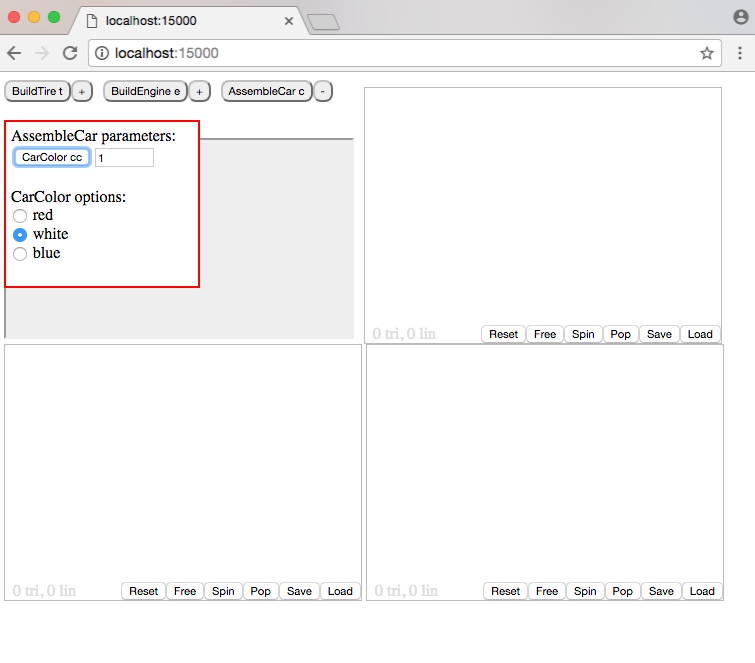
\includegraphics[width=0.75\textwidth]{pix/buttons3.png}
\caption{\f{WEBGUI} after calling \textbf{webinit} to create 3 command buttons, and 1 parameter with 3 options.}
\label{fig:12}
\end{figure} 

 \newpage
 \cleardoublepage
\setcounter{chapter}{3} %The counter for chapters should be set one less than 
                        %the actual chapter number, for example, {1} for 
                        %chapter 2, and {2} for chapter 3.
\setcounter{section}{4} %The counter for sections should be set to match the
                        %actual chapter number, for example, {2} for sections 
                        %in chapter, and {3} for sections in chapter 3. 
\chapter{GUI Features}
\markboth{WEBGUI USERS' GUIDE}{GUI FEATURES}
\pagenumbering{arabic}
\setcounter{page}{39} %The counter for page numbers must be placed here in your
                     %chapter, following the \chapter and \markboth commands.
                     %It should always be the next available right-hand page.
                     %All chapters start on new rights. It will always be
                     %an odd number.  

 
\section{Basic layout}
\begin{figure}[H]
\centering
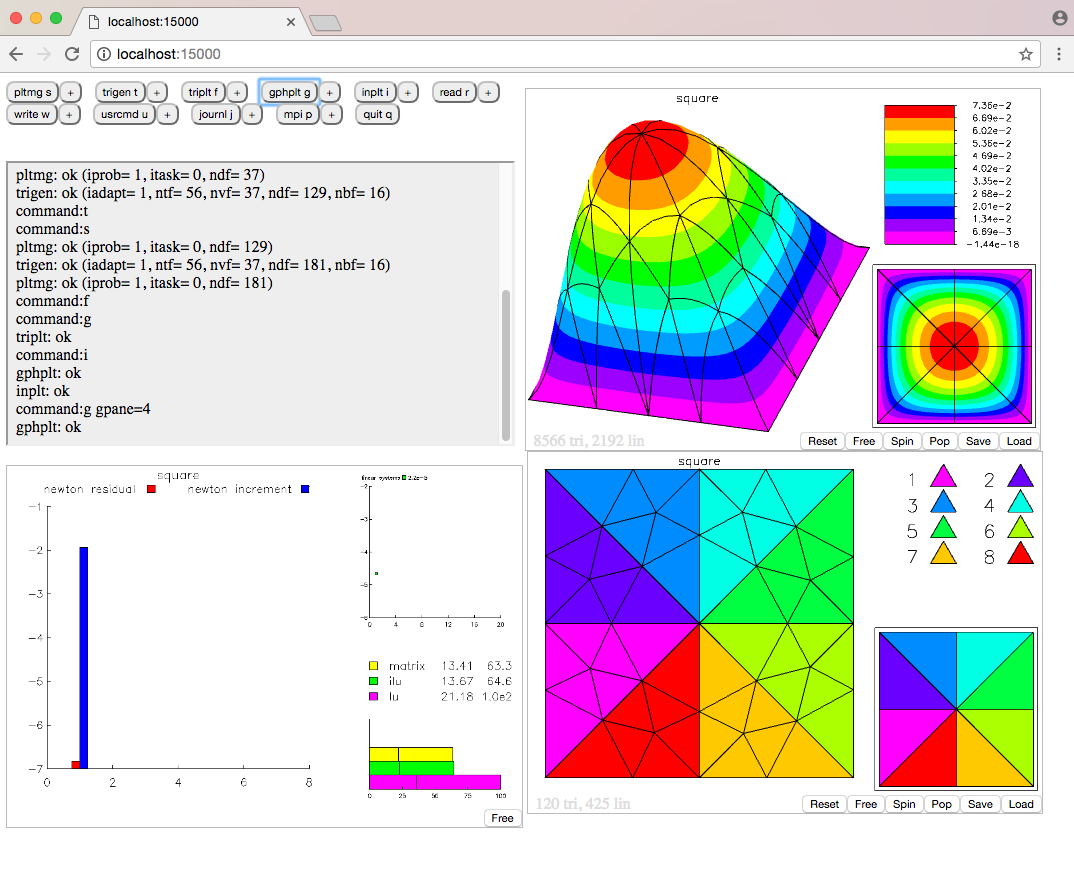
\includegraphics[width=0.75\textwidth]{pix/example2.png}
\caption{\f{WEBGUI}'s appearance in a web browser.}
\label{fig:4-1}
\end{figure} 
Above is an image of \f{WEBGUI} running together with Randolph Bank's software \f{PLTMG}. This picture illustrates
the basic features of \f{WEBGUI}'s graphic user interface. Randy's softare \f{PLTMG} called \textbf{webinit}
to define 11 buttons and many parameters and options. (To learn how to add buttons see Section \ref{sec:3-2}.)
Next it called \textbf{webstart}. After that a user opened a web browser and directed it to the host computer's URL. 
Then the user clicked some buttons issuing commands. \f{PLTMG} outputted many lines of text and one 2D
image and two 3D objects.

The web browser graphic interface is divided into 4 rectangle areas. The top left area contains the command buttons
and a pane to display text output. The text output pane also displays a history of the commands issued. A command is
issued whenever the user (i) presses a command button, (ii) closes a drop down menu after 
changing a parameter, or (iii) types a command into the command string field and hits enter. (If you wish for
your software to send text output to the text output pane, use the routine \textbf{webwriteline} described in Section 
\ref{sec:2-2}.)

The remaining 3 rectangle areas are panes numbered 0, 1, 2 (corresponding to the top right, bottom left, and 
bottom right pane)(they are also numbered 3, 4, 5). These panes are where 2D images and 3D objects (WebGL) 
outputted by software are displayed. Each
pane can display either one 2D image or one 3D object. Whenever a new image or object is sent to a pane, the old
image or object disappears and is replaced. (If you wish your software to send 2D images to a display pane, see Section 
\ref{sec:2-3}. To send 3D objects to a display pane, see Section \ref{sec:2-4}.)

\section{Display panes}
\label{sec:4-4}
The web browser interface has 3 display panes. Each display one 2D image or one 3D object. The display panes 
are numbered 0, 1, 2 corresponding to the top right, bottom left, bottom right (also numbered 3, 4, 5). In Figure \ref{fig:4-1},
pane 0(3) and 2(5) contain a 3D object. And pane 1(4) contains a 2D image.

3D objects are displayed using WebGL 1.0. Most web browsers and computers from the year 2010 onward have WebGL enabled
by default. When a 3D object is displayed, the user can rotate, pan, and zoom the object using their mouse. Rotate
using the left mouse button, pan using the middle mouse button, and zoom using the right mouse button. If your mouse
doesn't have a center button, you can push the "option" (on Mac) or "alt" (on Windows) key while using the left mouse button 
instead. If your mouse doesn't have a right button, you can push the "command" (on Mac) or "windows" (on Windows) key 
while using the left mouse button instead.

\begin{center}
\begin{tabular}{|l|l|l|l|}
\hline
\multicolumn{2}{|c|}{\strutul Display pane buttons} \\
\hline 
\strutul
Button & Effect \\
\hline
\strutu
RESET & return a zoomed / panned / rotated image to its initial state \\
FREE & clear the image and free associated memory \\
SPIN & spin image \\
POP & place canvas in its own web browser tab\\
PUSH & return canvas to its original location in the web browser tab\\
SAVE & save image to a file\\
LOAD & read image from a file\\
\hline
\end{tabular}
\end{center}

Under each 3D object are 6 buttons labeled Reset, Free, Spin, Pop, Save, and Load. Pressing the Reset button
returns the 3D object to its original location reseting any rotation, pan, or zoom information. 

Pressing Free, deletes the object and frees any memory associated with storing the object. See Section 
\ref{sec:5-1} to learn about \f{WEBGUI}'s memory usage. 

Pressing Spin allows the object to rotate freely. It will continue rotating in the direction that the user
last rotated. After pressing Spin, you will see a new button labeled Stop. Pressing Stop stops the object from rotating
freely. 

Pressing Pop places the current display pane in its own browser tab or window (depending on your web 
browser's settings). If your web browser places the pane in a new tab but you prefer a new window, either 
change your web browser's settings or open a new window and cut and paste the tab's URL into the new window.
When a display pane resides in its own tab or window, you will see a button labeled Push under the new pane. 
Pressing Push will put the display pane back into the main controls window.

Pressing Save will save a binary file with an extension of "gpu" to your local computer containing the 3D object's information.
This file can be loaded back into a display pane using the Load button.

Under each 2D image is only 1 button labeled Free. Pressing this button deletes the image and frees any memory
associated with storing the image. See Section \ref{sec:5-1} to learn about \f{WEBGUI}'s memory usage. 

\section{Quaternion rotation}
3D objects that are drawn to frame 5 can be rotated, panned, and zoomed with the mouse (explained in previous section). 
Objects in frames 1, 2, 3, 4 cannot.
Frame 5's viewing area is a cube with the coordinates of the lower left back $(0,0,0)$ and the upper right front $(1,1,1)$.
The center of this frame is coordinates $(0.5,0.5,0.5)$. See Figure \ref{fig:4-3}.

\begin{figure}[H]
\centering
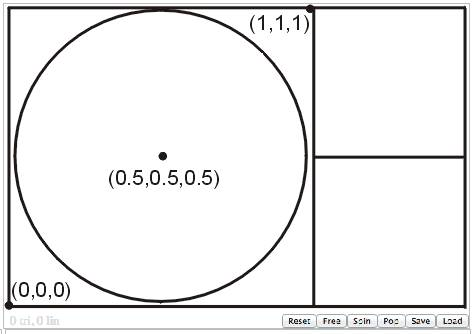
\includegraphics[width=0.75\textwidth]{pix/circle.jpg}
\caption{A 2D projection of a sphere in frame 5}
\label{fig:4-3}
\end{figure}

\begin{figure}[H]
\centering
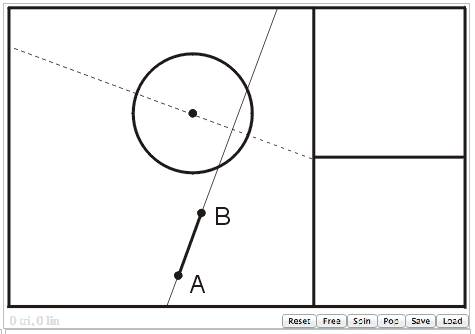
\includegraphics[width=0.75\textwidth]{pix/axis3.jpg}
\caption{Moving the mouse from $A$ to $B$ rotates the object in 3D around the dotted line axis.}
\label{fig:4-4}
\end{figure}

A 3D object gets rotated whenever a user depresses the left mouse button, moves the mouse, and then releases the
left mouse button. Rotation is calculated as follows. Imagine a sphere of radius $0.5$ that fills frame 5 with
center at $(0.5,0.5,0.5)$. Projected into 2D, this is a circle as shown in Figure \ref{fig:4-3}. The user can zoom and 
pan frame 5 moving the circle to a new size and location in the web browser. When a user depresses the left mouse button, 
call this point $A$. Then the user moves the mouse. Call the point where the user releases the left mouse button point $B$.
Projected into 2D, the line through the center of the circle perpendicular to line $AB$ is the axis
of 3D rotation. The axis is the dotted line in Figure \ref{fig:4-4}.

In 3D, the angle between the axis of rotation
and the $XY$ plane is $\alpha = sin^{-1}(d/r)$ where $r$ is the radius of the circle and 
$d$ is the distance between the center of the circle and
the line $AB$. If $d>r$ then $\alpha = \pi/2$. The above defines the axis of rotation $u$.
The amount of rotation in radians is $\theta = 3s/(2r)$ where $s$ is the distance from $A$ to $B$ and $r$ is the radius
of the circle. The associated quaternion to facilatate this rotation is 
$q=[cos(\theta /2), u_x sin(\theta /2), u_y sin(\theta /2), u_z sin(\theta /2)]$ when $u$ is normalized to length 1.

As the user holds down the left mouse button and moves the mouse between point $A$ and point $B$,
the mouse travels through points $C_k$ in between. For each point $C_k$, \f{WEBGUI} shows the user what the object would
look like if the user released the left mouse button at $C_k$. Therefore as the mouse moves, the object
appears to continually rotate. None-the-less, when the mouse button is released, the inbetween points $C_k$ are ignored
and the above formula is used to calculate the new orientation of the object.



\section{Control keys}
\label{sec:4-1}
\f{WEBGUI} has some features which are toggled with key strokes.
\begin{center}
\begin{tabular}{|l|l|l|l|}
\hline
\multicolumn{2}{|c|}{\strutul Control keys} \\
\hline 
\strutul
Key & Feature \\
\hline
\strutu
OPTION + C & toggles between command buttons and command text field \\
OPTION + I & toggles displaying rotation, pan, and zoom information \\
OPTION + R & toggles whether 3D objects inherit rotation, pan, and zoom\\
OPTION + W & toggles between 2 display panes wide and 1 pane wide \\
OPTION + F & toggles firewall on and off\\
OPTION + E & toggles endian flip on and off\\
OPTION + SAVE & saves 3D object as text instead of binary\\
\hline
\end{tabular}
\end{center}

To use the above features, you hold down the OPTION key while pressing the indicated key. On a Windows machine,
hold down the ALT key instead of the OPTION key.

OPTION + C toggles between command buttons and command text field. If your software calls \textbf{webinit} before
calling \textbf{webstart}, then your web browser GUI will have command buttons. Note that the command buttons are just
short cuts for generating and submitting command strings to the command string buffer. See Section \ref{sec:3-3} for an 
explanation. Therefore the buttons are never needed. If you prefer to type your own command strings, then you can
toggle the command buttons off and on with OPTION +C.

OPTION + I toggles displaying rotation, pan, and zoom information. When these keys are pressed, the 3D object display
pane that is in focus will display its current rotation, pan, and zoom information. Note that when a display pane contains
a 2D image, there is no rotation, pan, and zoom information to display for that display pane.

OPTION + R toggles whether 3D objects inherit the rotation, pan, and zoom setting from the previously displayed 3D object.
By default, when you display a new 3D object, it will display without any zoom, pan, or rotation applied even if you zoomed, 
panned, and rotated the previous 3D object that was in the same display pane. After you press OPTION + R, the web
browser will display a pop up message indicating the status of inheritance.

OPTION + W toggles the web browser's appearance between 2 display panes wide and 1 display pane wide. On mobile
devices the default is 1 display pane wide. On other devices the default is 2 display panes wide.

OPTION + F toggles the firewall on and off. When the firewall is activated, the bottom of the web browser will display the 
following line of text indicating this
\begin{verbatim}
FIREWALL ON: Only your ip address (X.X.X.X) can access webgui.
\end{verbatim}
and, on the server machine, the standard output will display
\begin{verbatim}
webgui: Only accepting ip address = X.X.X.X
\end{verbatim}
where x.x.x.x is your ip address. And when the firewall is turned off, the standard output will display
\begin{verbatim}
webgui: Accepting all ip addresses.
\end{verbatim}

OPTION + E toggles an endian flip on and off. All but one feature of \f{WEBGUI} are independent of whether the
server machine and client machine have the same endianness or not. The only feature that is affected is displaying
3D objects. 3D objects are sent between the server and client as a binary stream of 4 byte variables (either integers
or floating point numbers). By default, the client assumes that the server has the same endianness as itself. If this 
is not the case, then press OPTION + E, to toggle an endian flip to allow the correct display of 3D objects. When endian
flip is turned on, the bottom of the web browser will display the following line of text indicating this
\begin{verbatim}
ENDIAN FLIP: Client is receiving flipped endianness of server.
\end{verbatim}

OPTION + SAVE allows your computer to save a 3D object as ASCII text instead of a binary string of floating point
numbers. This allows you to view the 3D object and see the individual triangles and lines that make up the 
object. You can also view the colors of these triangles and lines. Currently, the Load button will not load the ASCII text
files. If you want to be able to load a saved 3D object, then press SAVE without holding down OPTION. This will
save the 3D object as a binary file and allow it to be loaded later.

\section{Miscelleanous}
\subsection{Display without controls}
\label{sec:4-2}

\f{WEBGUI} can be used another way. Instead of receiving user input and displaying software output, \f{WEBGUI}
can just be used to display output as show in Figure \ref{fig:4-2}. Notice how this is different than the normal appearance
in Figure \ref{fig:4-1}. To have your web browser perform this way, use the URL = "http:// localhost:15000/ sg?x=0" instead of 
URL = "http:// localhost:15000/ index.html". In place of $x=0$, choose $x=0$, $x=1$, or $x=2$ depending on which display pane 
you wish to view. And of course in place of "http:// localhost", you put the ip address of the host machine and in place of 
15000, you put the port that your web server is listening on. 

\begin{figure}[H]
\centering
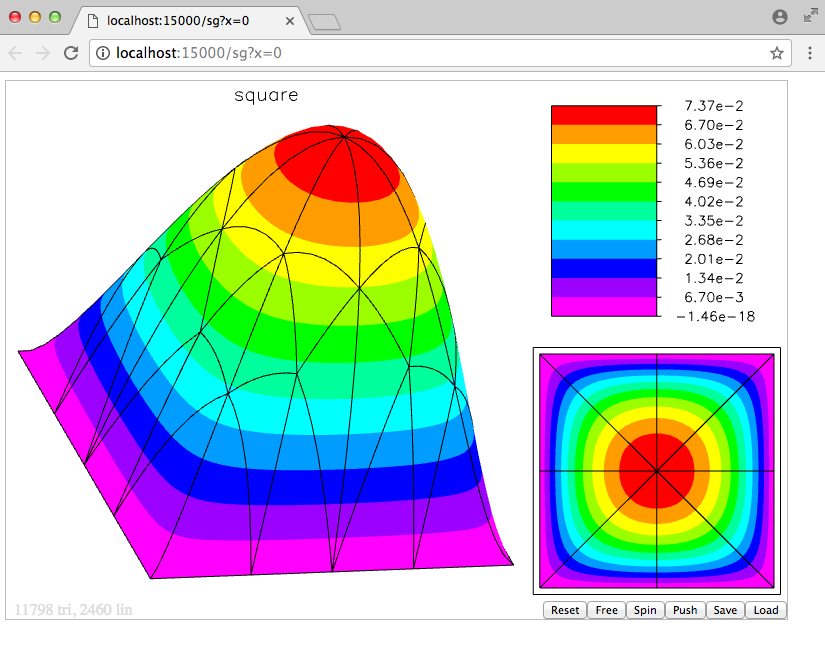
\includegraphics[width=0.75\textwidth]{pix/sg.png}
\caption{\f{WEBGUI} in display only mode by using a special URL.}
\label{fig:4-2}
\end{figure} 

\subsection{Save and view webpage offline}
\label{sec:4-3}

When you are viewing \f{WEBGUI} within your web browser, you may desire to save the web page so that you can 
view or edit the webpage offline. Of course at any time you can just select "Save page as" in your web browser. You can
even select "Save webpage complete". However if you do either of these and then open the saved files, they will not display
any 3D objects. If you wish to save a version that contains the 3D objects, there is a work around.

In your web browser, change the URL from "http:// localhost:15000/ index.html" to "http:// localhost:15000/ save". Of course
in place of "http:// localhost", you put the ip address of the host machine and in place of 15000, you put the port
that your web server is listening on. After entering this new URL, you will see what looks like the same web page. However,
if you choose "Save webpage complete" and reload it offline, you will see the 3D objects. This works because the 3D objects
will be stored as ASCII text data within a JavaScript file. This is recognized by your web browser and your web browser will
save it. Normally, the 3D objects are being stored as proprietary binary data which is must faster to transmit and load. But your
web browser does not recognize these binary files and won't save them. Only use the special save URL to save the web page;
\f{WEBGUI} will not operate correctly in save mode.

If you wish to save the appearance of a single 3D object (without the command buttons showing as displayed in Figure \ref{fig:4-2}), 
you have two choices. You can simply click the Save button
beneath the object you wish to save as explained in Section \ref{sec:4-4}. This saves a very small binary file. Or instead, 
you can go to the URL = "http:// localhost:15000/ save?x=0" which will allow you to view display pane 0 and save it by selecting
"Save webpage complete" from your web browser. Use $x=1$ or $x=2$ for display panes 1 and 2.


 \newpage
 \cleardoublepage
\setcounter{chapter}{4} %The counter for chapters should be set one less than 
                        %the actual chapter number, for example, {1} for 
                        %chapter 2, and {2} for chapter 3.
\setcounter{section}{5} %The counter for sections should be set to match the
                        %actual chapter number, for example, {2} for sections 
                        %in chapter, and {3} for sections in chapter 3. 
\chapter{WEBGUI Memory Usage}
\markboth{WEBGUI USERS' GUIDE}{WEBGUI MEMORY USAGE}
\pagenumbering{arabic}
\setcounter{page}{47} %The counter for page numbers must be placed here in your
                     %chapter, following the \chapter and \markboth commands.
                     %It should always be the next available right-hand page.
                     %All chapters start on new rights. It will always be
                     %an odd number.  

 
\section{Overview}
\label{sec:5-1}
When you compile and link \f{WEBGUI} to your software, upon running it shares the memory space of your software.
This section describes \f{WEBGUI}'s memory usage so that you are aware. There are five main consumers of memory.
Only one can really become significant which is displaying large 3D objects. 

\section{Basic}
Since webgui.c is a web server, the first use of memory is maintaining index.html in memory
to be ready whenever a web browser requests it. This is roughly 100,000 bytes. Next, if you call \textbf{webinit} and enable the
web browser to store parameters giving the user the ability to view and change parameters, these variables are stored. An average number
of command buttons, parameters, and options uses around 10,000 bytes. (Each parameter uses about 100 bytes and each command button 
uses about 50 bytes.) Next webgui.c maintains a few command string buffers; these buffers use a total of 25,000 bytes.

\section{2D Images}
The two large uses of memory are the display of 2D images and 3D objects. When a 2D image is displayed, webgui.c must keep a copy
of the image in memory even though it passes the data on to the web browser. If someone refreshes a web browser, then webgui.c must
serve up the image again. \f{WEBGUI} only allows 2D images to have a maximum of 255 colors, therefore each pixel consumes 1 byte in 
memory. Storing the palette doesn't use much memory. If your software displays a 1200 by 800 image (by calling \textbf{webimagedisplay}), 
then  1200 x 800 = 960,000 pixels were submitted. Thus this image uses
1 megabyte of memory. If the user viewing the web browser no longer needs the image, they can click a button labeled Free beneath the image
to free this 1 megabyte of memory in memory space.

\section{3D Objects}
\label{sec:5-2}
3D objects can require the most use of memory depending on how many polygons and lines make up the object. Whenever your software
calls \textbf{webline} thus sending a line with multiple vertices, the line is saved in webgui.c 's memory as separate line segments. 
When your software calls \textbf{webfill} thus sending a convex
polygon, the polygon is saved in webgui.c 's memory as separate triangles. Every line segment uses 32 bytes of memory and every triangle
uses 44 bytes of memory. Therefore if you send a large 3D object with one million line segments and one million triangles, then this object
will use 75 megabytes of memory. Even though webgui.c sends this data to the web browser, it keeps a copy of the object in memory in case
someone reloads a web page and a web page needs to receive the object again. At any time, a user can free this memory by clicking the
button labeled Free beneath the displayed 3D object.

Additionally webgui.c uses a large temporary block of memory for a few seconds. Every time \textbf{webline} is called,
then 32 more bytes are allocated for each line segment. Each time \textbf{webfill} is called, 44 bytes are used per triangle. 
This memory is allocated as the calls execute. The 3D
object isn't drawn until your software calls \textbf{webgldisplay}. When this function is called, then webgui.c allocates another temporary
block of memory equal in size to the combined memory usage of all the stored lines and triangles. For example, if one million lines
are submitted and one million triangles are submitted, then 75 megabytes of memory are allocated. When \textbf{webgldisplay} is called,
another 75 megabytes of memory is allocated (for 150 MB total). This additional 75 megabytes contains the data in a special format usable
by the GPU on the client's computer. This 75 MB is then transmitted to the client and then freed. (Afterward the server is only
using the original 75MB) Next, the web browser of the client's computer holds the 75 MB of data in memory for one second and then this 
data is passed into the client's GPU and the web browser frees the 75MB. The entire time
that the 3D object is visible on the client's screen, the GPU has the 75 MB in its memory and webgui.c has 75 MB in its memory.

These two 75 MB usages of memory are freed when the user clicks Free under the displayed 3D object, or when another 2D image or 3D object
is displayed in the same display pane. When a new 2D image or 3D object is sent to an already used display pane, then the data 
associated with the old image or object is freed and replaced by the new image or object.
 \newpage
 \cleardoublepage
\setcounter{chapter}{5} %The counter for chapters should be set one less than 
                        %the actual chapter number, for example, {1} for 
                        %chapter 2, and {2} for chapter 3.
\setcounter{section}{6} %The counter for sections should be set to match the
                        %actual chapter number, for example, {2} for sections 
                        %in chapter, and {3} for sections in chapter 3. 
\chapter{Example Driver}
\markboth{WEBGUI USERS' GUIDE}{EXAMPLE DRIVER}
\pagenumbering{arabic}
\setcounter{page}{49} %The counter for page numbers must be placed here in your
                     %chapter, following the \chapter and \markboth commands.
                     %It should always be the next available right-hand page.
                     %All chapters start on new rights. It will always be
                     %an odd number.  

 
\section{Overview}
This section contains an example driver written in C, that when compiled and linked to webgui.c creates a simple
program that lets a user draw lines and triangles. By modifying this example, you can create a program that uses
\f{WEBGUI} quickly. In the source code below, it is indicated which variables and functions
are general purpose and which are specific to this application. 

After running example.c and opening a web browser,
you are presented with the command buttons shown in Figure \ref{fig:6-1}. This figure also shows the drop down menu
for DrawTriangle visible. To draw a triangle, input the coordinates $(x1,y1,z1)$, $(x2,y2,z2)$, $(x3,y3,z3)$. Input 
the color as $(Red, Green, Blue)$ where $0 \leq R,G,B \leq 255$. Finally, input the pane and frame. 

\begin{figure}[H]
\centering
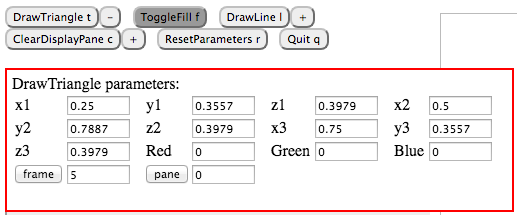
\includegraphics[width=0.75\textwidth]{pix/driver2.png}
\caption{example.c allows a user to draw lines and triangles. This figure shows the DrawTriangle drop down menu open.}
\label{fig:6-1}
\end{figure} 

If the ToggleFill button is highlighted then the triangle will be drawn unfilled. And if the ToggleFill button is not 
highlighted, the triangle will be filled. Press the ToggleFill button to toggle it.
The rest of the buttons are self explanatory. Figure \ref{fig:6-2} shows the result of drawing
4 unfilled triangles in 3D to create a tetrahedron. The image shows the tetrahedron after it has been rotated by
the user. The 4 vertices are drawn in $frame=5$ and positioned at $(0.25,0.3557,0.3979)$, $(0.5,0.7887,0.3979)$, 
$(0.75,0.3557,0.3979)$, $(0.5,0.5,0.8061)$. Note that $(0.5,0.5,0.5)$ is the center of rotation in $frame=5$.
In this example, the tetrahedron has edge length 0.5 and is centered at $(0.5,0.5,0.5)$.

\begin{figure}[H]
\centering
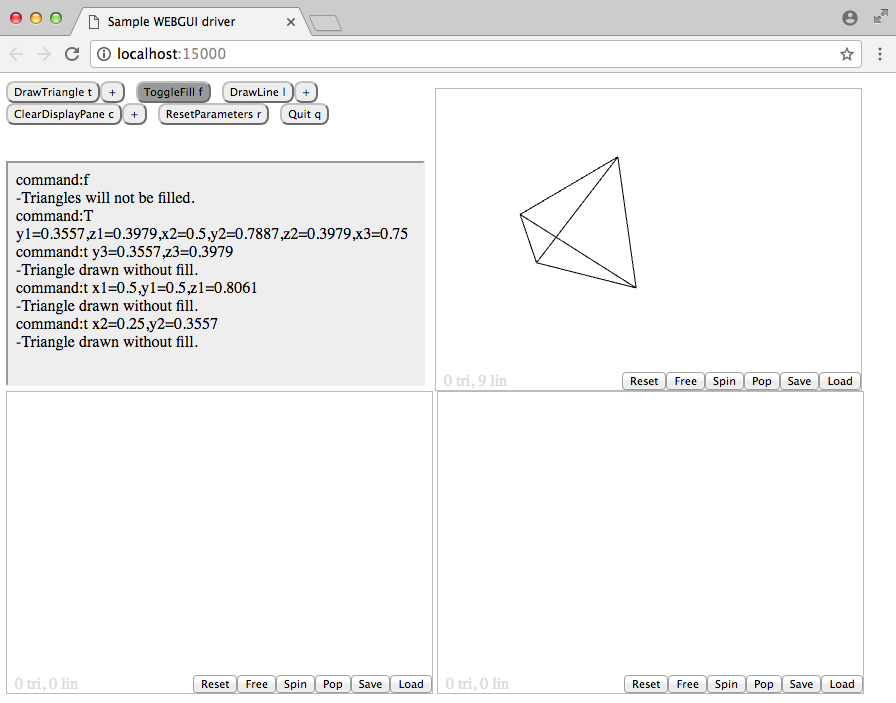
\includegraphics[width=0.75\textwidth]{pix/driver3.png}
\caption{example.c compiled with webgui.c. Then user draws a skeleton tetrahedron.}
\label{fig:6-2}
\end{figure} 

\section{Example driver source in C}
\begin{verbatim}
#include<stdio.h>
#include<stdlib.h>
#include<string.h>
#include<webgui.h>

/* general routines for any program using webgui.c */
void initParameterMap(char* str, int n);
char* extractVal(char* str, char key);
char processCommand(char* str);
void updateParameter(char* str, int index1, int index2);
char arrayGet(char* key);
int ipGet(char* key);
void ipSet(char* key, int value);
double rpGet(char* key);
void rpSet(char* key, double value);
char* spGet(char* key);
void spSet(char* key, char* value);
/* general variables */
int ct=0;
char** map_keys;
int* map_indices;
char* map_array;
double *rp_default, *rp;
int *ip_default, *ip;
char *sp_default, *sp;
char buffer[80];

/* program specific routines */
void drawTriangle();
void drawTriangleOutline();
void drawLine(int display);
void drawAllObjects(int pane);
void clearDisplay();
/* program specific variables */
char init[60][80]={
    "c c=DrawTriangle,k=t",
    "c c=ToggleFill, k=f",
    "c c=DrawLine,k=l",
    "c c=ClearDisplayPane, k=c",
    "c c=ResetParameters, k=r",
    "c c=Quit, k=q",
    "n n=x1, t=r, i=1, d=0.25",
    "n n=y1, t=r, i=2, d=0.25",
    "n n=z1, t=r, i=3, d=0.5",
    "n n=x2, t=r, i=4, d=0.75",
    "n n=y2, t=r, i=5, d=0.25",
    "n n=z2, t=r, i=6, d=0.5",
    "n n=x3, t=r, i=7, d=0.5",
    "n n=y3, t=r, i=8, d=0.75",
    "n n=z3, t=r, i=9, d=0.5",
    "n n=x4, t=r, i=10, d=0.25",
    "n n=y4, t=r, i=11, d=0.5",
    "n n=z4, t=r, i=12, d=0.5",
    "n n=x5, t=r, i=13, d=0.75",
    "n n=y5, t=r, i=14, d=0.5",
    "n n=z5, t=r, i=15, d=0.5",
    "n n=Red, t=i, i=1, d=0",
    "n n=Green, t=i, i=2, d=0",
    "n n=Blue, t=i, i=3, d=0",
    "n n=frame, t=i, i=4, d=5",
    "n n=pane, t=i, i=5, d=0",
    "r c=DrawTriangle, n=x1",
    "r c=DrawTriangle, n=y1",
    "r c=DrawTriangle, n=z1",
    "r c=DrawTriangle, n=x2",
    "r c=DrawTriangle, n=y2",
    "r c=DrawTriangle, n=z2",
    "r c=DrawTriangle, n=x3",
    "r c=DrawTriangle, n=y3",
    "r c=DrawTriangle, n=z3",
    "r c=DrawTriangle, n=Red",
    "r c=DrawTriangle, n=Green",
    "r c=DrawTriangle, n=Blue",
    "r c=DrawTriangle, n=frame",
    "r c=DrawTriangle, n=pane",
    "r c=DrawLine, n=x4",
    "r c=DrawLine, n=y4",
    "r c=DrawLine, n=z4",
    "r c=DrawLine, n=x5",
    "r c=DrawLine, n=y5",
    "r c=DrawLine, n=z5",
    "r c=DrawLine, n=Red",
    "r c=DrawLine, n=Green",
    "r c=DrawLine, n=Blue",
    "r c=DrawLine, n=frame",
    "r c=DrawLine, n=pane",
    "r c=ClearDisplayPane, n=pane",
    "s n=pane, v=0, l=\"0 top right\"",
    "s n=pane, v=1, l=\"1 bottom left\"",
    "s n=pane, v=2, l=\"2 bottom right\"",
    "s n=frame, v=1, l=\"1 all\"",
    "s n=frame, v=2, l=\"2 top right\"",
    "s n=frame, v=3, l=\"3 bottom right\"",
    "s n=frame, v=4, l=\"4 left\"",
    "s n=frame, v=5, l=\"5 rotate\""
};
float triangles[3][1000], lines[3][700];
int indexT[3]={0,0,0}, indexL[3]={0,0,0};
double red[3][200], green[3][200], blue[3][200];
int fill=1;

int main(int argc, char *argv[]){
    int i, offset=0; 
    char cmd, str[80];
    initParameterMap((char*)init,60);
    webinit((char*)init,60);
    websettitle("Sample WEBGUI driver");
    while (webstart(15000+offset)<0) offset++;
    while (1){
        webreadline(str);
        cmd = processCommand(str);
        if (cmd=='t'){
            if (fill==1){
                drawTriangle();
                webwriteline("-Triangle drawn with fill.");
            }
            else{
                drawTriangleOutline();
                webwriteline("-Triangle drawn without fill.");
            }
        }
        else if (cmd=='f'){
            fill *= -1;
            if (fill==1){
                webwriteline("-Triangles will be filled.");
                webbutton(0,"ToggleFill");
            }
            else {
                webwriteline("-Triangles will not be filled.");
                webbutton(1,"ToggleFill");
            }
        }
        else if (cmd=='l'){
            drawLine(1);
            webwriteline("-Line drawn.");
        }
        else if (cmd=='c'){
            clearDisplay();
            webwriteline("-Display pane cleared.");
        }
        else if (cmd=='r'){
            webupdate(ip_default,rp_default,sp_default);
            for (i=0;i<ct;i++){
                ip[i] = ip_default[i];
                rp[i] = rp_default[i];
                strcpy(sp+80*i, sp_default+80*i);
            }
            webwriteline("-Parameters reset.");
        }
        else if (cmd=='q'){
            webwriteline("-Quitting.");
            webstop();
            return 0;
        }
    }
    return 0;
}
void initParameterMap(char* str, int n){
    /* reads array of strings and initializes ip, rp, sp */
    /* and creates a map for accessing ip, rp, and sp */
    int i, index=0;
    for (i=0; i<n; i++) if (str[80*i]=='n') ct++;
    map_keys = (char**)malloc(ct * sizeof(char*));
    map_indices = (int*)malloc(ct * sizeof(int));
    map_array = (char*)malloc(ct * sizeof(char));
    rp_default = (double*)malloc(ct * sizeof(double));
    ip_default = (int*)malloc(ct * sizeof(int));
    sp_default = (char*)malloc(ct * sizeof(char*) * 80);
    rp = (double*)malloc(ct * sizeof(double));
    ip = (int*)malloc(ct * sizeof(int));
    sp = (char*)malloc(ct * sizeof(char*) * 80);
    for (i=0; i<ct; i++) map_keys[i] = (char*)malloc(20 * sizeof(char));
    for (i=0; i<n; i++)
    if (str[80*i]=='n'){
        strcpy(map_keys[index],extractVal(str+80*i,'n'));
        map_indices[index] = atoi(extractVal(str+80*i,'i'))-1;
        map_array[index] = *extractVal(str+80*i,'t');
        if (map_array[index]=='r'){
            rp_default[map_indices[index]] = atof(extractVal(str+80*i,'d'));
            rp[map_indices[index]] = rp_default[map_indices[index]];
        }
        else if (map_array[index]=='i'){
            ip_default[map_indices[index]] = atoi(extractVal(str+80*i,'d'));
            ip[map_indices[index]] = ip_default[map_indices[index]];
        }
        else if (map_array[index]=='s'){
            strcpy(sp_default+80*map_indices[index],extractVal(str+80*i,'d'));
            strcpy(sp+80*map_indices[index],sp_default+80*map_indices[index]);
        }
        index++;
    }
}
char* extractVal(char* str, char key){
    /* returns the value associated with key in str */
    buffer[0]=0;
    int index1 = 0, index2;
    while (index1<strlen(str)){
        if (str[index1]=='='){
            if (str[index1-1]==key){
                index2 = index1;
                while (index2<strlen(str) && str[index2]!=',') index2++;
                strncpy(buffer,str+index1+1,index2-index1-1);
                buffer[index2-index1-1]=0;
                break;
            }
        }
        index1++;
    }
    return buffer;
}
char processCommand(char* str){
    /* returns command char and updates parameters */
    int index1 = 1, index2 = 2;
    while (str[index2]!=' '){
        if (str[index2]==','){
            updateParameter(str,index1,index2);
            index1 = index2;
        }
        index2++;
    }
    if (index2>2) updateParameter(str,index1,index2);
    return str[0];
}
void updateParameter(char* str, int index1, int index2){
    /* parses str between index1 and index2 and updates parameter */
    int index3 = index1+1;
    while (str[index3]!='=') index3++;
    str[index2]=0; str[index3]=0;
    char ch = arrayGet(str+index1+1);
    if (ch=='r') rpSet(str+index1+1,atof(str+index3+1));
    else if (ch=='i') ipSet(str+index1+1,atoi(str+index3+1));
    else if (ch=='s') spSet(str+index1+1,str+index3+1);
    str[index2]=','; str[index3]='=';
}
char arrayGet(char* key){
    /* returns which array (ip, rp, sp) key belongs to */
    int i;
    char value = ' ';
    for (i=0; i<ct; i++) if (strcmp(map_keys[i],key)==0)
        value = map_array[i];
    return value;
}
int ipGet(char* key){
    int i, value = 0;
    for (i=0; i<ct; i++) if (strcmp(map_keys[i],key)==0)
        value = ip[map_indices[i]];
    return value;
}
void ipSet(char* key, int value){
    int i;
    for (i=0; i<ct; i++) if (strcmp(map_keys[i],key)==0)
        ip[map_indices[i]] = value;
    return;
}
double rpGet(char* key){
    int i;
    double value = 0;
    for (i=0; i<ct; i++) if (strcmp(map_keys[i],key)==0)
        value = rp[map_indices[i]];
    return value;
}
void rpSet(char* key, double value){
    int i;
    for (i=0; i<ct; i++) if (strcmp(map_keys[i],key)==0)
        rp[map_indices[i]] = value;
    return;
}
char* spGet(char* key){
    int i;
    buffer[0] = 0;
    for (i=0; i<ct; i++) if (strcmp(map_keys[i],key)==0)
        strcpy(buffer,sp + 80 * map_indices[i]);
    return buffer;
}
void spSet(char* key, char* value){
    int i;
    for (i=0; i<ct; i++) if (strcmp(map_keys[i],key)==0)
        strcpy(sp + 80 * map_indices[i],value);
    return;
}
void drawTriangle(){
    int i, j;
    char str[3], var[3]={'x','y','z'};
    int pane = ipGet("pane");
    /* save triangle data locally */
    triangles[pane][indexT[pane]*10 + 9] = ipGet("frame");
    for (int i=1;i<4;i++)
    for (int j=0;j<3;j++){
        sprintf(str,"%c%d",var[j],i);
        triangles[pane][indexT[pane]*10+3*(i-1)+j] = (float)rpGet(str);
    }
    red[pane][indexT[pane]] = ipGet("Red")/255.0;
    green[pane][indexT[pane]] = ipGet("Green")/255.0;
    blue[pane][indexT[pane]] = ipGet("Blue")/255.0;
    indexT[pane]++;
    /* draw all triangles and lines to pane */
    drawAllObjects(pane);
}
void drawTriangleOutline(){
    int i, j;
    double x4=rpGet("x4"), y4=rpGet("y4"), z4=rpGet("z4");
    double x5=rpGet("x5"), y5=rpGet("y5"), z5=rpGet("z5");
    char str[3], str2[3], var[3]={'x','y','z'};
    for (i=4;i<6;i++)
    for (j=0;j<3;j++){
        sprintf(str,"%c%d",var[j],i);
        sprintf(str2,"%c%d",var[j],i-3);
        rpSet(str, rpGet(str2));
    }
    drawLine(0);
    for (i=4;i<6;i++)
    for (j=0;j<3;j++){
        sprintf(str,"%c%d",var[j],i);
        sprintf(str2,"%c%d",var[j],i-2);
        rpSet(str, rpGet(str2));
    }
    drawLine(0);
    for (j=0;j<3;j++){
        sprintf(str,"%c4",var[j]);
        sprintf(str2,"%c1",var[j]);
        rpSet(str, rpGet(str2));
    }
    for (j=0;j<3;j++){
        sprintf(str,"%c5",var[j]);
        sprintf(str2,"%c3",var[j]);
        rpSet(str, rpGet(str2));
    }
    drawLine(1);
    rpSet("x4",x4); rpSet("y4",y4); rpSet("z4",z4);
    rpSet("x5",x5); rpSet("y5",y5); rpSet("z5",z5);
}
void drawLine(int display){
    int i, j;
    char str[3], var[3]={'x','y','z'};
    int pane = ipGet("pane");
    /* save line data locally */
    lines[pane][indexL[pane]*7 + 6] = ipGet("frame");
    for (int i=4;i<6;i++)
    for (int j=0;j<3;j++) {
        sprintf(str,"%c%d",var[j],i);
        lines[pane][indexL[pane]*7+3*(i-4)+j] = (float)rpGet(str);
    }
    red[pane][100+indexL[pane]] = ipGet("Red")/255.0;
    green[pane][100+indexL[pane]] = ipGet("Green")/255.0;
    blue[pane][100+indexL[pane]] = ipGet("Blue")/255.0;
    indexL[pane]++;
    /* draw all triangles and lines to pane */
    if (display==1) drawAllObjects(pane);
}
void drawAllObjects(int pane){
    int i, j;
    float x[3], y[3], z[3];
    websetcolors(200,red[pane],green[pane],blue[pane],pane);
    for (i=0;i<indexT[pane];i++){
        webframe((int)triangles[pane][i*10+9]);
        for (j=0;j<3;j++){
            x[j] = triangles[pane][10*i+3*j];
            y[j] = triangles[pane][10*i+3*j+1];
            z[j] = triangles[pane][10*i+3*j+2];
        }
        webfillflt(x,y,z,3,i+1);
    }
    for (i=0;i<indexL[pane];i++){
        webframe((int)lines[pane][i*7+6]);
        for (j=0;j<2;j++){
            x[j] = lines[pane][7*i+3*j];
            y[j] = lines[pane][7*i+3*j+1];
            z[j] = lines[pane][7*i+3*j+2];
        }
        weblineflt(x,y,z,2,i+101);
    }
    webgldisplay(pane);
}
void clearDisplay(){
    int pane = ipGet("pane");
    indexL[pane]=0;
    indexT[pane]=0;
    websetcolors(200,red[pane],green[pane],blue[pane],pane);
    webgldisplay(pane);
}
\end{verbatim}

\section{Example driver source in Fortran}




 \newpage
 \cleardoublepage
\setcounter{chapter}{6} %The counter for chapters should be set one less than 
                        %the actual chapter number, for example, {1} for 
                        %chapter 2, and {2} for chapter 3.
\setcounter{section}{7} %The counter for sections should be set to match the
                        %actual chapter number, for example, {2} for sections 
                        %in chapter, and {3} for sections in chapter 3. 
\chapter{Modifying WEBGUI}
\markboth{WEBGUI USERS' GUIDE}{MODIFYING WEBGUI}
\pagenumbering{arabic}
\setcounter{page}{59} %The counter for page numbers must be placed here in your
                     %chapter, following the \chapter and \markboth commands.
                     %It should always be the next available right-hand page.
                     %All chapters start on new rights. It will always be
                     %an odd number.  

\section{Introduction}
\label{sec:6-1}
This is an advanced section. Most users will never need to read this section. You do not need to read this 
section in order to use \f{WEBGUI} as a front end for your software. Everything you need to know about using
\f{WEBGUI} is contained in previous sections. Only read this section if you have special needs and would like
to customize or alter \f{WEBGUI}'s normal behavior.

\section{Overview}
\f{WEBGUI} is copyrighted by its author. It is ok to modify \f{WEBGUI} to your particular application
but please give credit to its author and note your modifications. This section helps explain how to modify \f{WEBGUI}. 
Since \f{WEBGUI} is basically a web server, modifying \f{WEBGUI} requires changing the default index.html file also.
Unlike ordinary web servers where this file is a separate file on the hard drive, \f{WEBGUI} contains
this file as data within its C code as an array of strings.

In the distribution of \f{WEBGUI}, we provide you with the file index.html as its own file and this section
explains how to modify it and place the contents back into webgui.c as data. Or alternatively this section
shows you how you can run webgui.c with an external index.html file. Additionally, \f{WEBGUI} displays
3 png images which are contained within the C code as an array of unsigned char.

Also to assist in customizing \f{WEBGUI} to your needs, this Chapter explains three more things; the 
communication between webgui.c and the web browser,  the private variables and functions of \f{WEBGUI}, 
and how WebGL works in both the web browser and webgui.c.

\section{index.html}
\label{sec:7-4}
The main task of \f{WEBGUI} is to be the front end for software and must receive input from the user and display output.
\f{WEBGUI} accomplishes this by utilizing a web page in a web browser. It creates a web page by mimicking a web server 
and then provides the file \textbf{index.html} to the client's web browser. On the client's side, the file \textbf{index.html} contains 
instructions to create a web page with buttons to receive input and display panes to show output. \textbf{index.html} contains
JavaScript code to allow the web page to be interactive and employs AJAX techniques. \textbf{index.html} also uses
HTML, CSS, and WebGL for formatting and display. On the server side, \textbf{webgui.c} mimics a web server, PHP processing,
and a MySQL database. \textbf{webgui.c} also interacts directly with software during runtime which 
is written in C or Fortran.

Whenever a web browser requests \textbf{index.html} it is created dynamically and then communicated as a string of characters. 
Within \textbf{webgui.c}, the file \textbf{index.html} is the concatenation of four string variables \textbf{webpageA}, \textbf{webpageB}, 
\textbf{webpageC}, and \textbf{webpageD}. Variable \textbf{webpageA} contains the beginning of \textbf{index.html} and the 
instructions to create the command buttons and input elements
to display and change parameters. \textbf{webpageB} contains instructions to create drop down menus to present options
for parameters. \textbf{webpageC} contains the overall layout of the web page and provides all the functionality. \textbf{webpageC}
is the majority of \textbf{index.html} and contains all the JavaScript, CSS, and WebGL. \textbf{webpageD} contains history information.
When you first load \textbf{index.html}, \textbf{webpageD} is mostly blank. If you reload your browser during your session,
then \textbf{webpageD} contains instructions to recreate the history of your session.

Every time a web browser requests \textbf{index.html}, \textbf{webpageA} is created fresh. Since \textbf{webpageA} contains
input elements to display parameters, \textbf{webpageA} must be updated at the time of a request to contain the current
parameter values. The portion \textbf{webpageB} is created once when \textbf{webinit} is called and never changed.
The portion \textbf{webpageC} is loaded once when \textbf{webstart} is called and never changed. Every time a web
browser requests \textbf{index.html}, \textbf{webpageD} is created fresh. Since \textbf{webpageD} contains the session 
history, \textbf{webpageD} must be updated to contain the current history. The web browser receives these four strings
consecutively and thinks it is receiving the one file \textbf{index.html}.

If you wish to change the appearance or function of the web page in the web browser, you must alter \textbf{index.html}.
To alter \textbf{index.html}, you must change the four pieces,  \textbf{webpageA}, \textbf{webpageB}, \textbf{webpageC}, 
and \textbf{webpageD}. To do this, you must alter the functions that build the pieces.
The piece \textbf{webpageA} is created in the function \textbf{updatewebpageA} within \textbf{webgui.c}.
In order for \textbf{webpageA} to create command buttons and work with parameters, it references the variables that 
contain information about commands and parameters. This information is contained in variables like \textbf{cmdn},
\textbf{cmda}, \textbf{cmdt} and \textbf{nn}, \textbf{na}, \textbf{nd}, etc. These variables are explained in Section \ref{sec:7-1}
below. 

The piece \textbf{webpageB} is created in the function \textbf{webinit}. The piece \textbf{webpageC} doesn't need to be created.
Instead it is loaded from either the hard drive or data within \textbf{webgui.c}. The next Section \ref{sec:7-2} explains this.
Finally, the piece \textbf{webpageD} is created in the function \textbf{updatewebpageD}. Section \ref{sec:4-2} explains how
\f{WEBGUI} can be used to display output only and not receive user input. That version of \textbf{index.html} uses a different
\textbf{webpageD} which gets created in the function \textbf{updatewebpageD2}.

Note that the best way to view \textbf{index.html} is to run \textbf{webgui.c} after linked to your software and then from your
web browser choose "View Source". (Google search "how to view a web page's source" if you don't know how to do this).
This will display the entire \textbf{index.html}. The beginning is \textbf{webpageA}. Following that is \textbf{webpageB} and 
\textbf{webpageC}. And the ending is \textbf{webpageD}. As a beginning point
of changing \f{WEBGUI}, you could save this file to your hard drive and start changing this file, reloading it, and seeing the consequence.
The best way to save \f{WEBGUI}'s webpage to a file is explained in Section \ref{sec:4-3}.

\section{External versus internal}
\subsection{indexC.html}
\label{sec:7-2}
The portion of \textbf{index.html} called \textbf{webpageC} is contained in the data variable \textbf{char indexhtml[x][y]} 
located at the end of \textbf{webgui.c}. This is an array of $x$ strings with each string having a maximum length of $y$. These
strings are the lines of the file \textbf{indexC.html} which resides on the hard drive. Since this data is within \textbf{webgui.c}, the
file \textbf{indexC.html} is not needed to run \f{WEBGUI}. The file \textbf{indexC.html} is only helpful if you wish to modify
\f{WEBGUI}.

If you wish to change the function or appearance of \f{WEBGUI}'s web page, then you can set the variable \textbf{load\_webpageC\_from\_file}
equal to 1. Afterward, make changes to the file \textbf{indexC.html}, and each time you quit and run \textbf{webgui.c}, it will load 
the new updated \textbf{indexC.html} from the hard drive. (You do not need to recompile \textbf{webgui.c} between trials). Once the web page 
appears and behaves as you like, you should place the file \textbf{indexC.html} within \textbf{webgui.c} as data. To do this,
you must convert each line into a string by placing quotation marks around it. And any quotation marks inside the line must have
a backslash added before. Any backslash needs an additional backslash before it. And care must be taken to convert the carriage
returns correctly. The easiest way to convert \textbf{indexC.html} into the array of strings \textbf{char indexhtml[x][y]} is to run
the program \textbf{convert2str.c}. It reads in \textbf{indexC.html} and writes the array of strings into \textbf{output.txt}. It also tells
you how many strings there are and the maximum length of these strings. Cut and paste the contents of \textbf{output.txt} into
\textbf{webgui.c}. Next, correct the value of \textbf{clines} in the function \textbf{updatewebpageC} to match \textbf{[x]}, the number of
strings. Finally, set the variable \textbf{load\_webpageC\_from\_file} equal to 0.

As an alternative to moving the contents of the file \textbf{indexC.html} within \textbf{webgui.c}, you can leave the variable
\textbf{load\_webpageC\_from\_file} equal to 1 and leave the file \textbf{indexC.html} in \textbf{webgui.c} local directory.

\subsection{png images}
\f{WEBGUI}'s web page displays 3 png images. A typical web server would have these images reside on the hard drive.
In the case of \textbf{webgui.c}, these images reside within the code of \textbf{webgui.c} as data. Specifically, they are the variables
\textbf{unsigned char folderpng[446]}, \textbf{unsigned char uppng[472]}, and \textbf{unsigned char filepng[402]}. In the web page,
these images appear when a user opens the drop down menu to select a file as shown in Figure \ref{fig:7-1}.

\begin{figure}[H]
\centering
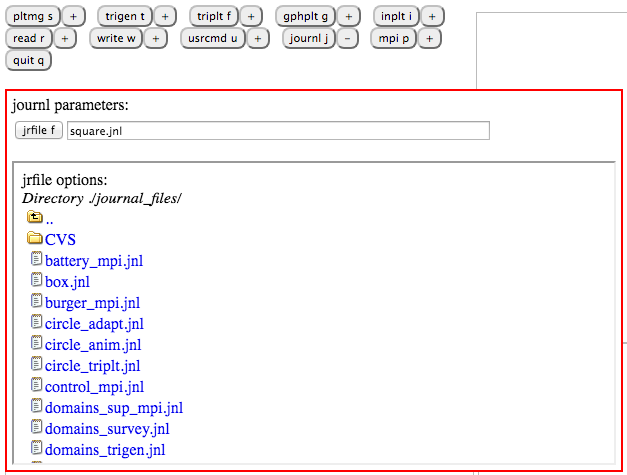
\includegraphics[width=0.75\textwidth]{pix/png.png}
\caption{User is selecting a file. Down the left side are png images. This figure shows WEBGUI interfaced with PLTMG.}
\label{fig:7-1}
\end{figure} 

In Figure \ref{fig:7-1}, the three png images named \textbf{up.png}, \textbf{folder.png}, \textbf{file.png} are shown to the left of the
blue words. These 3 files are provided with the distribution of \textbf{webgui.c} as external files. As explained above, they are not
needed to run \textbf{webgui.c} because their data is within \textbf{webgui.c}. These external files are provided in case a user
wishes to modify these images and/or make new ones.

If you wish to change the function or appearance of \f{WEBGUI}'s png images, then you can set the variable 
\textbf{load\_pngs\_from\_file} equal to 1. Afterward, make changes to the files \textbf{up.png}, \textbf{folder.png}, \textbf{file.png}, 
and each time you quit and run \textbf{webgui.c}, it will load 
the new updated files from the hard drive. (You do not need to recompile \textbf{webgui.c} between trials). Once the web page 
appears as you like, you should place the files within \textbf{webgui.c} as data. A png image 
file is just a sequence of byes (unsigned char). Therefore to place the data within \textbf{webgui.c}, just write these bytes as numbers 
in the declaration of the appropriate variable.

The easiest way to convert \textbf{up.png}, \textbf{folder.png}, \textbf{file.png} into an array of unsigned char is to run
the program \textbf{convert2int.c}. It reads in the png files and writes an array of unsigned char into \textbf{output.txt}. The usage for
\textbf{convert2int.c} is \textbf{convert2int source\_file}. After running \textbf{convert2int.c}, cut 
and paste the contents of \textbf{output.txt} into \textbf{webgui.c}. Finally, set the variable \textbf{load\_pngs\_from\_file} equal to 0.
 
As an alternative to moving the contents of \textbf{up.png}, \textbf{folder.png}, \textbf{file.png} within \textbf{webgui.c}, you can leave the variable
\textbf{load\_pngs\_from\_file} equal to 1 and leave the files \textbf{up.png}, \textbf{folder.png}, \textbf{file.png} in \textbf{webgui.c} local directory.

\section{Internal variables}
\label{sec:7-1}

\textbf{webgui.c} has many internal variables and functions. In this section, we will highlight the variables that
may be of interest to the reader wishing to modify \f{WEBGUI}. Important functions are highlighted in other sections when they
are relevant.

When software uses \textbf{webgui.c}, the first function that is called
is \textbf{webinit}. This function is explained in Section \ref{sec:2-1} and Section \ref{sec:3-1}. The purpose of calling \textbf{webinit}
is to add features to \f{WEBGUI}'s web page. Calling \textbf{webinit} can create command buttons and declare parameters. 
Declared parameters can be viewed and modified in the web page.

When \textbf{webgui.c} creates the web page, it references the declared parameters and requested command buttons. Information
about commands and parameters are stored in the following variables
\begin{verbatim}
static int cmdct, nct;
static const int maxnamelen=20, maxabbrlen=3, maxdeftlen=40;
static char **cmdn, **cmda, **cmdt;
static char **nn, **na, **nd, *nt;
static int **cmdp, *cmdpct, *cmdc;
static int *no, *nu, *nw, *ni;
\end{verbatim}

The above variables get initialized within the function call to \textbf{webinit}. All the variables that begin with the letter c reference
commands and all variables that begin with n reference parameters. Below are descriptions.\\
\textbf{const int maxnamelen=20, maxabbrlen=3, maxdeftlen=40} is the length of strings for name, abbreviation, and default values.\\
\textbf{int cmdct} is the quantity of commands.\\
\textbf{char** cmdn} is an array of strings equivalent to \textbf{char cmdn[cmdct][maxnamelen]} containing the full command names.\\
\textbf{char** cmda} is an array of strings equivalent to \textbf{char cmda[cmdct][maxabbrlen]} containing the abbreviated command names.\\
\textbf{char** cmdt} is an array of strings equivalent to \textbf{char cmdt[cmdct][maxnamelen]} containing the command types. Currently
this variable is initialized but unused.\\
\textbf{int* cmdpct} is an array equivalent to \textbf{int cmdpct[cmdct]} containing the quantities of parameters associated with each
command.\\
\textbf{int** cmdp} is an array equivalent to \textbf{int cmdp[cmdct][nct]} containing the indices of the parameters associated with each
command. Note that \textbf{nct} minus \textbf{cmdpct} elements are unused for each \textbf{cmdp[cmdct]}.\\
\textbf{int* cmdc} is an array equivalent to \textbf{int cmdc[cmdct]} containing 1 or -1 whether the respective command button is 
highlighted or not.\\
\textbf{int nct} is the quantity of parameters.\\
\textbf{char** nn} is an array of strings equivalent to \textbf{char nn[nct][maxnamelen]} containing the full parameter names.\\
\textbf{char** na} is an array of strings equivalent to \textbf{char na[nct][maxabbrlen]} containing the abbreviated parameter names.\\
\textbf{char** nd} is an array of strings equivalent to \textbf{char nd[nct][maxdeftlen]} containing the default parameter values. Note
that integer and real default values are stored as strings.\\
\textbf{char* nt} is an array of chars equivalent to \textbf{char nt[nct]} containing the parameter types (either i, r, s, l, or f).\\
\textbf{int* ni} is an array equivalent to \textbf{int ni[nct]} containing each parameter's index into their respective type's array.\\
\textbf{int* no} is an array equivalent to \textbf{int no[nct]} containing 1 or 0 whether the respective parameter has an options list.\\
\textbf{int* nu} is an array equivalent to \textbf{int nu[nct]} containing 1 or 0 whether the respective parameter is special. Ignore
this variable. Most likely your software will not use it.\\
\textbf{int* nw} is an array equivalent to \textbf{int nw[nct]} containing 1 or 0 whether the respective parameter is associated with 
a command or not.\\

Other important variables are
\begin{verbatim}
static const int maxlines = 100, maxhistory=100;
static int indexA = 0, indexB = 0;
static char *bufferA, *bufferB; //maintained as Fortran strings (space padded)
static char **history; //maintained as C strings (null terminated)

static char *webpageA, *webpageB, *webpageC, *webpageD;
static int load_webpageC_from_file = 1;
static int load_pngs_from_file = 1;

static float **colorsGL[3]={NULL,NULL,NULL};
static int ncolorGL[3]={0,0,0};
static float **triangles[3]={NULL,NULL,NULL};
static float **lines[3]={NULL,NULL,NULL};
static int indexT[3]={0,0,0}, indexL[3]={0,0,0};
static char *databuffer=NULL;
\end{verbatim}

The top group are explained in Section \ref{sec:7-3} below. The middle group are explained in Section \ref{sec:7-4} above.
The bottom group are explained in Section \ref{sec:7-5} below.

\section{Buffers and communication}
\label{sec:7-3}

\subsection{Overview}
The purpose of \f{WEBGUI} is to provide a front end for software. On behalf of software, \f{WEBGUI} receives input and displays output.
All input is in the form of command strings of maximum length 80. Output takes three forms. Output is either text, 2D images, 
or 3D objects. Output text is in the form of a string of maximum length 80. This section discusses input and output
strings and their communication. The following Sections \ref{sec:7-6} and \ref{sec:7-5} discuss the output of 2D images and 3D objects.

When a command button is pressed in the web browser of \f{WEBGUI}, the web page creates a command string and transmits
it to \f{webgui.c}. This command string waits in a command string buffer until the software requests it with a call to \textbf{webreadline}.
Software outputs text by calling \textbf{webwriteline(char* str)}. The outputted string waits in an output string buffer until the
web page requests it with an AJAX call. Therefore to facilitate input and output, buffers need to be maintained and strings need to
be transmitted between \f{webgui.c} (the web server) and the web page.

Software talks to \textbf{webgui.c} (directly via calls to \textbf{webreadline} and \textbf{webwriteline}), and \textbf{webgui.c} (the web server) 
talks to the web browser (via sockets and AJAX). All communication between a web browser and a web server (\textbf{webgui.c}) must be initiated 
by the web browser. And, all a web browser knows to do is request a URL. Whenever the web browser has a command string to pass on to the 
web server, the browser makes an AJAX request to the URL = http://localhost:15000/writeline.php?cmd='STR' where STR is replaced by the
command string of maximum length 80. And localhost:15000 is replaced by the host's ip address and listening port. In order for the 
web browser to receive output text from the web server, it continually asks if any text is available by making an AJAX request every half
second to URL = http://localhost:15000/readline.php . Each time, the web server responds with either an empty string, or a string of length 80. 
Every string that the web browser receives from readline.php, is displayed in the output text display pane with an appended html carriage return 
($<$br$>$).

\begin{verbatim}
static const int maxlines = 100, maxhistory=100;
static int indexA = 0, indexB = 0;
static char *bufferA, *bufferB; //maintained as Fortran strings (space padded)
static char **history; //maintained as C strings (null terminated)
\end{verbatim}

Above are internal variables within \textbf{webgui.c}.
Buffer B contains outputted text from the software. And buffer A contains command strings from the web browser. Each buffer
is an array of strings equivalent to \textbf{char buffer[maxlines][80]}. The variables \textbf{indexA} and \textbf{indexB}
track how many strings are in each queue. The software reads strings from bufferA and afterward they are removed from the queue.
The web browser reads strings from bufferB and afterward they are removed from the queue. A record of all strings is maintained
in a third array of strings named \textbf{char history[maxhistory][90]}. This is required in case the user refreshes the web browser.
If the web browser is reloaded and a new \textbf{index.html} is requested, then the web server must write the history of all previous commands 
and outputted text in the web page's output text display pane.

\subsection{Communication protocall}

The web browser and \textbf{webgui.c} (web server) pass strings back and forth. Every time a user
clicks a command button, the web browser sends a command string to the web server. Whenever a user closes a parameter drop
down menu after changing a parameter, the web browser sends a special capital letter command string (explained in Section \ref{sec:3-4}.)
Every time software has text to output, it calls \textbf{webwriteline} and the outputted string gets transmitted to the web browser.

In addition to the above three uses of strings, sometimes the web server needs to give the web browser special instructions. And sometimes
the web browser needs to give the web server special instructions. Whenever the web server needs to give the web browser a special
instruction, it places a number sign before the string. Below is an example.
\begin{verbatim}
#update,a=2,b=3.5,c=1
\end{verbatim}
Normally, the web browser assumes a received string is output text and displays it in the output text display pane. Whenever
the web browser sees a string that begins with a number sign, it doesn't display it. Instead it interprets it as a special instruction.
The web page's JavaScript function \textbf{processcmd(str)} (found in \textbf{indexC.html}) processes all special instructions.
The example above instructs the web browser to update (change) the value of parameters \textbf{a, b, c} to 2, 3.5, and 1 respectively.
Other special instructions are \textbf{image, webgl2, button, pause, start, unhide, lock, update, files}. The first two, instruct the 
web browser to request a waiting 2D image or 3D object. The next two highlight a command button and ask the user to click a
continue button. The last one, lists files on the web server's hard drive.

The web browser assumes that each received string is length 80. 
If a special instruction requires a longer string, it prefaces a string with a 
number sign followed by a number to indicate the number of length 80s it requires. For example
\begin{verbatim}
#3#update,key1=value1,key2=value2,etc
\end{verbatim}
The above example tells the web browser to expect that a string of length $240 = 80 \times 3$ is to follow. 

Whenever the web browser needs to give the web server a special instruction, it uses AJAX to contact the URL = http://
localhost:15000/callfunct.php?CMD=VAR where CMD is replaced with the desired special instruction and VAR is replaced with
the special instruction's variable(s). Within \textbf{webgui.c}, special instructions are processed within the routine 
\textbf{void *startlisten(void *arg)}. The special functions that are currently implemented are \textbf{continue, listfiles, release,
updateall, push, query, firewall, endian}.   

\section{2D Images}
\label{sec:7-6}

When software has an 2D image to output, it calls \textbf{websetcolors} and \textbf{webimagedisplay}. Afterward, \textbf{webgui.c}
notifies the web browser by sending a special instruction string
\begin{verbatim}
#image,WIDTH,HEIGHT,PANE
\end{verbatim}
where WIDTH and HEIGHT are replaced by the image's width and height. And PANE is replaced by the desired display pane.
Next, the web browser requests the image by requesting the resource \textbf{figure0.bmp}, \textbf{figure1.bmp}, or
\textbf{figure2.bmp} from the web server in a normal web browser - web server image request.

\section{3D Objects (WebGL)}
\label{sec:7-5}

When software has an 3D object to output, it calls \textbf{websetcolors, webframe, webline, webfill, webgldisplay}. Afterward, \textbf{webgui.c}
notifies the web browser by sending a special instruction string
\begin{verbatim}
#webgl2,PANE
\end{verbatim}
where PANE is replaced by the desired display pane.
Next, the web browser requests the 3D object by requesting the resource \textbf{data0.gpu}, \textbf{data1.gpu}, or
\textbf{data2.gpu} from the web server in a normal web browser - web server file request.

The "file" \textbf{dataX.gpu} is a binary data block. This block of memory is created in \textbf{webgui.c}'s function 
\textbf{int updatedatabuffer3(int x, int endian)}, then transmitted, then the memory is freed.
This "file" can be thought of as a sequence of numbers further divided into 3 sections; header, vertices, colors.

The first 80 bytes of \textbf{dataX.gpu} is the header which indicates the layout and length of the next two sections (vertices and colors).
The header is a sequence of 20 integers (4 bytes each). The first integer is the number of triangles
to draw in frame 5. The next integer is the number of lines to draw in frame 5.
The next 3 thru 10 integers are the number of triangles then lines for frames 3, 2, 4, 1 respectively. 
Integers 11 thru 20 are the numbers of triangles and lines declaring color information for frames 5, 3, 2, 4, 1 respectively.

Following the 20 integers (header section) is a sequence of 4 byte single precision floating point numbers. First come all the coordinates of the vertices for describing 
the triangles for frame 5. Each triangle is described by a sequence of 9 floating point numbers $(x1,y1,z1), (x2,y2,z2), (x3,y3,z3)$. 
Note that 1 triangle is 3 vertices is 9 coordinates.
Next come the coordinates of the vertices describing the lines for frame 5. Each line is described by a sequence of 6 floating point numbers,
$(x1,y1,z1), (x2,y2,z2)$.
Then triangles for frame 3, then lines frame 3, etc. Then frame 2, 4, 1.
 
Following the many coordinate floating point numbers (vertices section) is a sequence of 1 byte unsigned chars.
Each vertex has its own color and colors are 3 bytes, one unsigned char for each red, green, blue. Thus, if there 
are 10 triangles for frame 5 that require color declaration, then 90 unsigned chars are needed to describe the associated colors.
For example, a triangle's coordinates are 36 bytes as 9 floating point numbers, $(x1,y1,z1), (x2,y2,z2), (x3,y3,z3)$ 
and if that triangle declares colors then 9 bytes are needed as 9 unsigned chars, $(R1,G1,B1), (R2,G2,B2), (R3,G3,B3)$.

Therefore if \textbf{data[0]} is the first integer in \textbf{dataX.gpu} and \textbf{data[1]} is the second integer, then the size of \textbf{dataX.gpu}
in bytes equals the sum of the sizes of its three sections, (header) + (vertices) + (colors) which equals\\ 
$$\bigg(80\bigg) + \bigg(36 \sum_{k=0}^{4}data[2k] + 24 \sum_{k=0}^{4}data[2k +1]\bigg) + \bigg(9 \sum_{k=5}^{9}data[2k] + 6 \sum_{k=5}^{9}data[2k +1]\bigg).$$
This block of data is communicated to the web browser from
the web server. Then the web browser transmits this block of data (unaltered) into the client's GPU to display as WebGL.

For a given frame, usually the number of objects that declare colors (in colors section) is the same as the number of objects to 
be drawn (in vertices section) as in $data[k]=data[k+10]$ for $0\leq k \leq 9$. 
However, whenever all line colors are black for a particular frame then the associated $data[2k+1]$ for $5 \leq k \leq 9$ will equal 0
and the web browser and GPU know how to deal with that. (This saves bandwidth and memory.)

\subsection{Internal variables}

The "file" \textbf{dataX.gpu} only exists in \textbf{webgui.c}'s memory for a few seconds. When the software requests to display a 3D object by
calling \textbf{webgldisplay}, this temporary "file" is created in the variable \textbf{char *databuffer}, transmitted to the web browser, and then the 
memory is freed. This procedure is explained in Section \ref{sec:5-2}.

The permanent storage of a 3D object is stored in the following internal \textbf{webgui.c} variables:
\begin{verbatim}
static float **colorsGL[3]={NULL,NULL,NULL};
static int ncolorGL[3]={0,0,0};
static float **triangles[3]={NULL,NULL,NULL};
static float **lines[3]={NULL,NULL,NULL};
static int indexT[3]={0,0,0}, indexL[3]={0,0,0};
\end{verbatim}

Each time software calls \textbf{webline}, a new entry is added to \textbf{float **lines[3]}. In this triple array, \textbf{lines[0], lines[1], lines[2]}
are the lines for display panes 0, 1, 2 respectively. For display pane 0, \textbf{lines[0]} is equivalent to \textbf{lines[indexL[0]][8]} where
\textbf{indexL[0]} is the quantity of lines in display pane 0. Each line is represented by 8 floating point numbers. The first 6 are the 6 coordinates
of the 2 line segment endpoints, $(x0,y0,z0)$ and $(x1,y1,z1)$. The 7th float is the color (as an index reference to the color palette) and the 8th 
is the frame the line belongs to.

Each time software calls \textbf{webfill}, a new entry is added to \textbf{float **triangles[3]}. In this triple array, \textbf{triangles[0], triangles[1], 
triangles[2]} are the triangles for display panes 0, 1, 2 respectively. For display pane 0, \textbf{triangles[0]} is equivalent to 
\textbf{triangles[indexT[0]][11]} where \textbf{indexT[0]} is the quantity of triangles in display pane 0. Each triangle is represented by 11 floating point 
numbers. The first 9 are the 9 coordinates of the 3 triangle vertices, $(x0,y0,z0)$, $(x1,y1,z1)$, and $(x2,y2,z2)$. The 10th float is the color (as an index 
reference to the color palette) and the 11th is the frame the triangle belongs to.

The color palette is stored in the variables \textbf{float **colorsGL[3]} and \textbf{int ncolorGL[3]}. The color palette for display pane 0 is stored 
in the variable \textbf{colorsGL[0]} and is equivalent to \textbf{colorsGL[ncolorGL[0]][3]}. The variable \textbf{ncolorGL[0]} is the quantity of colors
in the palette of display pane 0, and each color is stored as 3 floating point numbers referring to the quantities of red, green, blue pigment.



 \newpage

\cleardoublepage
\setcounter{page}{133}
\markboth{WEBGUI USERS' GUIDE}{REFERENCES}
 \bibliography{ref}
 \bibliographystyle{siam}
%\newpage

\cleardoublepage
\setcounter{page}{139}
\markboth{WEBGUI USERS' GUIDE}{INDEX}
\flushbottom
 \printindex


\end{document}




